\documentclass[11pt]{article}
\usepackage[T1]{fontenc}
\usepackage{lmodern}
\usepackage[a4paper,margin=2.6cm]{geometry}
\usepackage{amsmath,amssymb,amsthm,mathtools}
\usepackage{microtype}
\usepackage{booktabs}
\usepackage{graphicx}
\usepackage{enumitem}
\usepackage[font=small,labelfont=bf]{caption}
\usepackage[hidelinks]{hyperref}
\hypersetup{pdftitle={Exact optimal dispatching to two fluid queues: closed form, heavy traffic and stochastic evidence},pdfauthor={Anonymous}}
\usepackage{xcolor}
\usepackage{framed}
\setlist{nosep,leftmargin=*}
\graphicspath{{../figures/}}
\numberwithin{equation}{section}
\newtheorem{theorem}{Theorem}
\newtheorem{lemma}[theorem]{Lemma}
\newtheorem{proposition}[theorem]{Proposition}
\newtheorem{corollary}[theorem]{Corollary}
\theoremstyle{definition}
\newtheorem{definition}[theorem]{Definition}
\theoremstyle{remark}
\newtheorem{remark}[theorem]{Remark}
\newcommand{\E}{\mathbb{E}}
\newcommand{\Prob}{\mathbb{P}}
\newcommand{\one}{\mathbf{1}}
\newcommand{\cx}{\le_{\mathrm{cx}}}
\DeclareMathOperator{\sgn}{sgn}
\emergencystretch=2em

\title{Exact optimal dispatching to two fluid queues:\\ closed form, heavy traffic and stochastic evidence}
\author{Anonymous}
\date{\small 23 October 2026. Version 1.0.0-candidate (unrefereed). DOI: \href{https://doi.org/10.5281/zenodo.23586955}{10.5281/zenodo.23586955}.\\
\small Code and data: \url{https://github.com/ipitchford/fluid-queue-optimal-dispatch}}

\begin{document}
\maketitle

\begin{abstract}
\noindent
Xie, Hyyti\"a and Righter introduced a fluid model of size-aware dispatching to parallel first-come first-served servers and conjectured that, with two servers, the relative workload imbalance increases along every optimal trajectory. We solve their two-server problem exactly. For every nonnegative mean-one size law that is not concentrated at one point, a single quadrature of the mean-absolute-deviation function $D(h)=\E|S-h|$ gives the optimal value function, the optimal state-feedback policy and the optimal path from every initial state. In words: jobs smaller than a cutoff go to the shorter queue and larger jobs to the longer one; the cutoff depends only on the relative imbalance and rises as the queues drift apart; once one queue is empty it is kept exactly busy when $\rho\ge1/2$, while at lower load it receives every job and stays empty. The verification argument allows idling, reflection at empty queues, atoms and unbounded support. It proves the conjecture as posed (sizes with a density) and extends it to all nondegenerate laws, with uniqueness of the optimal workload path. We also derive the heavy-traffic limit $(1-\rho)V\to\bar P\,x^2$, where $\bar P$ is the fraction of jobs, taking the largest first, that carries half the work; for continuous size laws $\bar P=\Prob(S\ge m)$, with $m$ the work median. This corrects a factor in the source's Proposition~3 and agrees exactly with the heavy-traffic constant of the CARD policy of Xie, Grosof and Scully. Further results are an exact rational controller for finite size laws, certified bounds and an implementable bin policy, an exact enclosure for an infinite-variance Pareto law, and the cost of noisy size estimates. In seeded simulations of the stochastic two-server system, the fluid rule used directly beats join-the-shortest-workload by 40--70\% for highly variable sizes but fails badly at high load for low-variability sizes. A stabilised version with a safety band repairs this and is competitive with tuned CARD and Dice. The simulations are numerical evidence only.
\end{abstract}

\noindent\textbf{Keywords:} size-aware dispatching; fluid queues; optimal control; verification theorem; heavy traffic; convex order.

\section{Introduction}\label{sec:intro}

A dispatcher sends each arriving job to one of two identical first-come first-served (FCFS) servers. It sees the job's size and both workloads. Which rule minimises the total waiting time? Even with Markovian arrivals and sizes no simple optimal rule is known for this size- and state-aware problem. Xie, Hyyti\"a and Righter \cite{XHR2026} (XHR below) therefore studied a fluid version: jobs arrive as a continuum of particles of different sizes, a large initial backlog drains deterministically, and the aim is to route the incoming fluid so that the total waiting cost of arriving jobs is as small as possible. They showed that shorter jobs should go to the shorter queue, reduced the two-server problem to a one-dimensional variational problem, computed optimal paths numerically, and stated the following conjecture.

\begin{framed}
\noindent\textbf{The conjecture.} In XHR, Section~5, the conjecture reads: \emph{``We conjecture that the optimal $\hat y'\ge0$ (the relative imbalance should increase for the optimal path).''} Section~6.1 restates it in words: \emph{``the relative imbalance always increases along any optimal trajectory to the origin (or until one queue empties).''}
\end{framed}

\noindent Here $\hat y=(u_1-u_2)/(u_1+u_2)$ is the relative imbalance. In XHR's Section~5 a prime denotes $d/dx$, where $x=u_1+u_2$ is the total backlog. Because $x$ decreases in forward time, the inequality read literally says that the imbalance does \emph{not} increase as the backlog drains. The parenthesis and the sentence of Section~6.1 say the opposite, and so do XHR's figures. We prove the forward-time statement: along every optimal path $z=\hat y$ increases strictly in time, so $dz/dx<0$ almost everywhere. The literal inequality $\hat y'\ge0$ is therefore false for every nondegenerate law. We read it as a sign convention or slip and resolve the verbal conjecture.

XHR assume sizes with a density. Under that assumption the conjecture holds without qualification (Theorem~\ref{thm:monotone}). We extend it to every nondegenerate law, with atoms and singular parts allowed. Deterministic sizes lie outside XHR's hypotheses. For them the conclusion fails, as XHR's own Proposition~5 already suggests: every work-conserving size-blind policy is then equally good (Section~\ref{sec:det}).

\begin{framed}
\noindent\textbf{The optimal policy in one paragraph.} Let $z\in[0,1]$ be the relative imbalance. While both queues hold work, compute a cutoff $h=Z^{-1}(z)$ from one scalar function $Z$ of the size law and load. Send jobs smaller than $h$ to the shorter queue and jobs larger than $h$ to the longer queue. When the queues are equal, send all incoming work to one of them. When one queue is empty and the load exceeds $1/2$, send it the smallest jobs, splitting an atom if necessary, so that it receives work at exactly its service rate $1/2$. When the load is at most $1/2$, send everything to the empty queue. Along the resulting path the cutoff rises, the queues drift apart, and the shorter queue empties in finite time.
\end{framed}

\paragraph{Main results.} The status of each statement is given in brackets.
\begin{enumerate}[label=(\roman*)]
\item \emph{Exact value and policy} (Theorems~\ref{thm:value}--\ref{thm:unique}; proved). For every nondegenerate mean-one law and every load $0<\rho<1$, an explicit function $V$ is the minimum cost among all admissible controls, including idling ones. The policy above attains it, and the optimal labelled workload path is unique (two mirror images at a tied start).
\item \emph{The conjecture} (Theorem~\ref{thm:monotone}; proved). Along every optimal path the relative imbalance is nondecreasing, and strictly increasing while both queues are positive and unequal.
\item \emph{Heavy traffic} (Theorem~\ref{thm:ht}; proved). $(1-\rho)V_\rho(x,y)\to\bar P x^2$ uniformly, where $\bar P$ is the fraction of jobs, taking the largest first and splitting an atom at the work median if needed, that carries half the work. For continuous size laws $\bar P=\Prob(S\ge m)$, where $m$ is the work median ($\E[S;S<m]=1/2$). Balanced routing has limit $x^2/2$. The ratio $2\bar P$ equals the ratio of the heavy-traffic constants of CARD and least-work-left in the stochastic system \cite{XGS2024}. XHR's Proposition~3, as printed, has an extra factor $2\rho$ in its axis term. Correcting it removes a factor~2 from their heavy-traffic limit.
\item \emph{Computation and approximation} (Theorems~\ref{thm:finite}, \ref{thm:wass}, Propositions~\ref{prop:envelope}--\ref{prop:noisy}; proved). For finite support the value is piecewise quadratic, with an exact rational recurrence. Convex-order discretisation gives two-sided bounds and a bin policy with certified regret. The value is Lipschitz in the Wasserstein distance with a constant independent of the law. For a Pareto law with infinite variance we give an exact rational enclosure. Routing on noisy size estimates is optimal-equivalent to routing on a coarser size law.
\item \emph{Stochastic system} (Section~\ref{sec:sim}; numerical evidence only). In seeded simulations of the two-server queue, the fluid rule used directly beats join-the-shortest-workload by a wide margin for highly variable sizes, but is much worse for exponential and two-point sizes at high load. A stabilised rule with a safety band repairs most of this and is competitive with tuned CARD and Dice; for two-point sizes no rule gains more than 9\% over JSW.
\end{enumerate}

\begin{table}[t]
\centering\small
\caption{What XHR established and what is added here (two servers).}\label{tab:xhr}
\begin{tabular}{@{}p{0.43\textwidth}p{0.5\textwidth}@{}}
\toprule
XHR \cite{XHR2026} & This paper\\
\midrule
Short jobs to the short queue (Prop.~1); scale invariance (Lemma~2, Cor.~2--3). & Used. The closed form follows quickly from their variational problem (Section~\ref{sec:heuristic}).\\
Variational problem $\min\int(1-2\Phi(y'))y\,dx$; numerical optimal paths. & Closed-form value and policy for all nondegenerate laws; global verification over all admissible controls, including idling and reflection (Section~\ref{sec:proof}).\\
Monotone imbalance or a straight-to-origin (STO) path (Cor.~4); conjecture of increasing imbalance. & Conjecture proved; strict increase; no STO segment in the interior and no balanced dwelling is ever optimal; unique optimal path (Section~\ref{sec:allopt}).\\
Most-work-left value (Prop.~3) and heavy-traffic limit. & Corrected value and limit; heavy-traffic theorem for the optimum; agreement with CARD (Section~\ref{sec:ht}).\\
Convex-order monotonicity (Prop.~4). & Direct proof via an envelope formula; certified brackets; Wasserstein stability; noisy sizes (Section~\ref{sec:approx}).\\
Size-blind equivalence (Prop.~5). & Exact deterministic value; the equivalence needs $\rho\ge1/2$ (Section~\ref{sec:det}).\\
Heuristics F-BLB, F-blbh tested in simulation. & Simulation of the exact rule and of a stabilised rule against JSW, SITA, Dice and CARD (Section~\ref{sec:sim}).\\
\bottomrule
\end{tabular}
\end{table}

\paragraph{How much is new.} Once XHR's variational problem is written down, the Beltrami first integral gives the candidate in a few lines (Section~\ref{sec:heuristic}). We say so plainly. The work lies in proving that the candidate is optimal against \emph{every} admissible control, including non-work-conserving and idling controls, at every load. The proof must handle reflected axes, the kink on the diagonal, atoms, unbounded support and infinite horizons. It must also identify all optimal controls, which is what the conjecture's quantifier requires. Beyond this we add the heavy-traffic theorem and its reconciliation with the stochastic literature, exact and certified computation, and a simulation study.

\paragraph{Running example.} Throughout, \emph{the running example} has sizes $1/2$ and $3/2$ with probability $1/2$ each, load $\rho=3/4$ and initial workloads $(1/2,1/2)$. Its optimal cost is $33/28\approx1.179$. Balanced routing, which here means random splitting, join-the-shortest-workload or load-balanced SITA, costs $3/2$; the saving is $3/14\approx21\%$. Figure~\ref{fig:twopoint} shows the optimal path. All incoming work first goes to one queue. After the imbalance reaches $3/13$, small jobs go to the shorter queue. Once that queue is empty it takes all small jobs and $5/9$ of the large ones.

\begin{figure}[t]
\centering
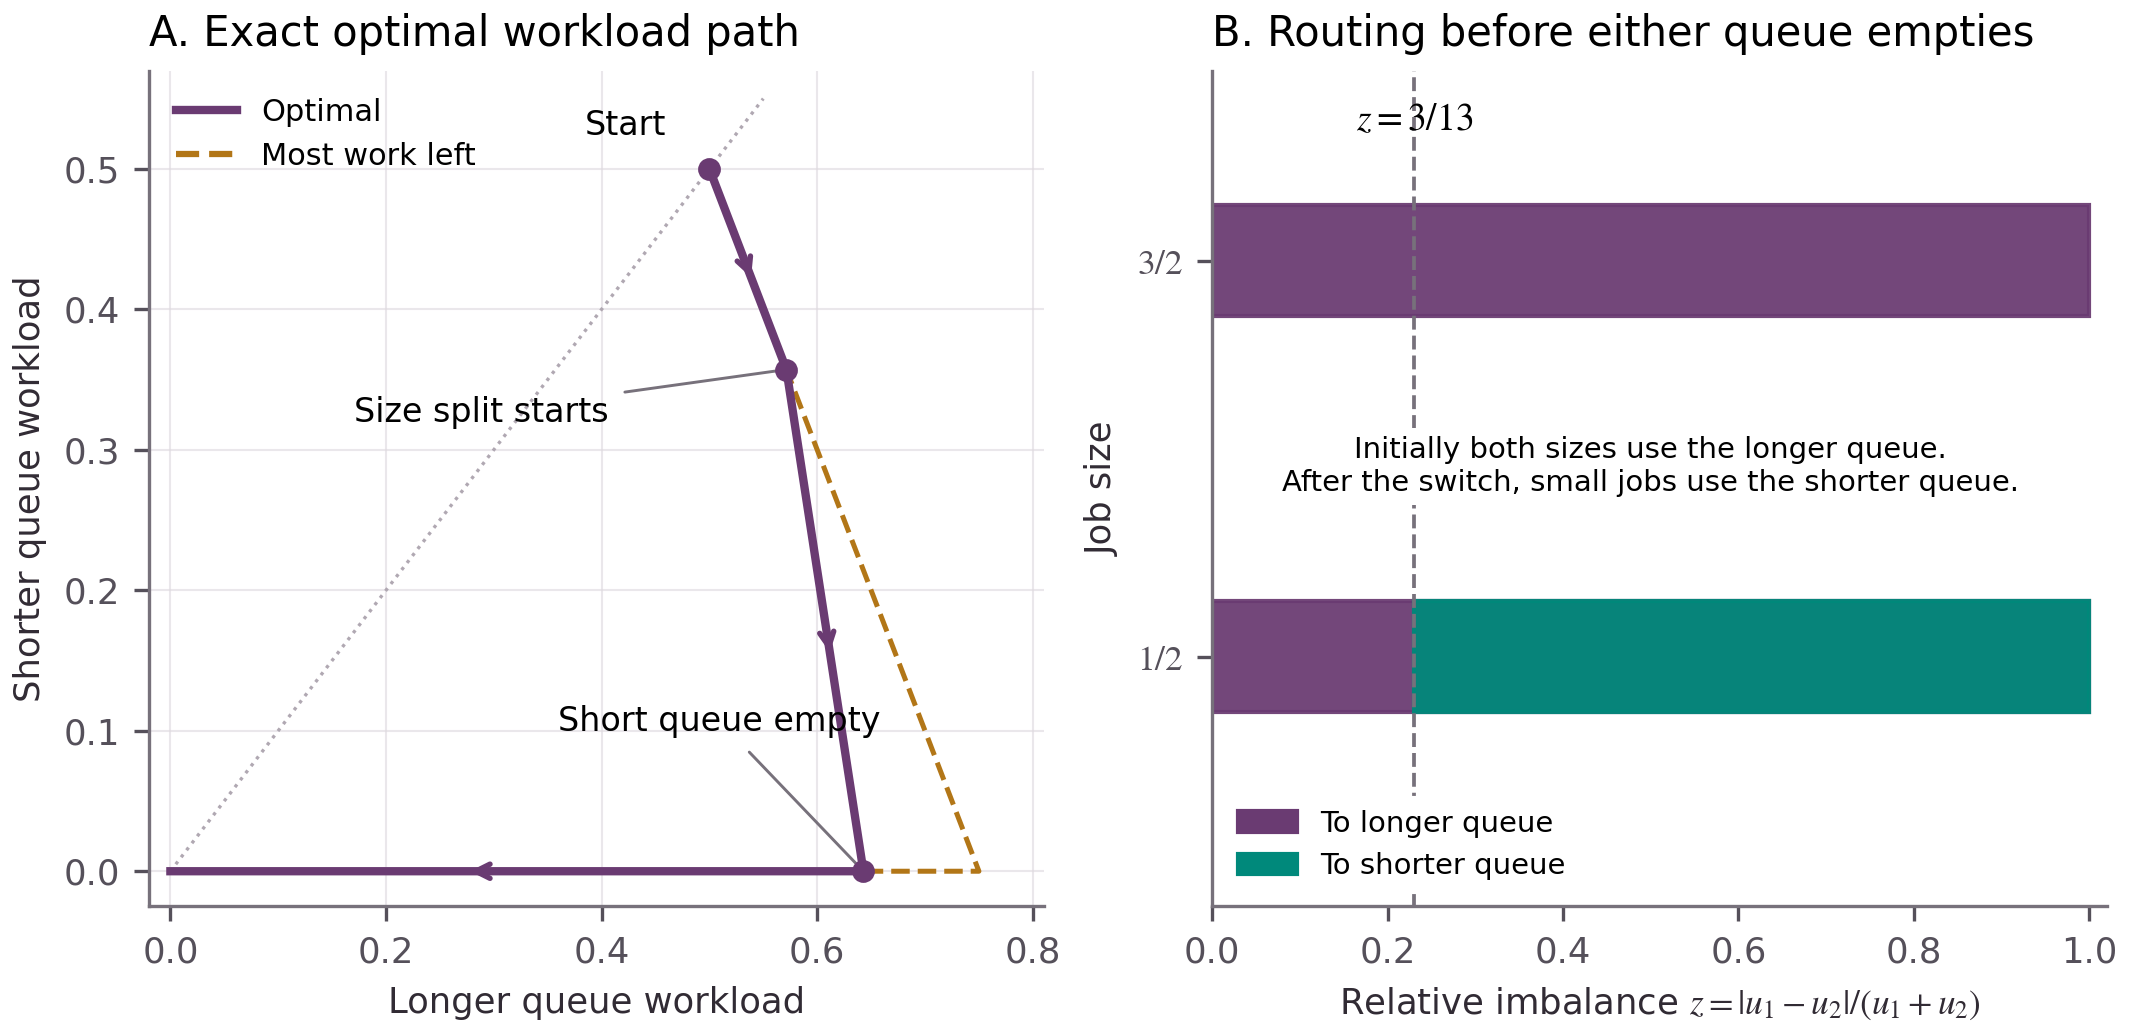
\includegraphics[width=\linewidth]{two_point_policy.png}
\caption{The running example (sizes $1/2,3/2$ equally likely, $\rho=3/4$, start $(1/2,1/2)$). Left: the optimal workload path (cost $33/28$) and most-work-left (cost $21/16$). Balanced routing stays on the diagonal and costs $3/2$. Right: routing by size before either queue empties; the partition changes at $z=3/13$.}\label{fig:twopoint}
\end{figure}

\paragraph{Related work.} \emph{Dispatching.} With state information only, joining the shortest queue or least work left is optimal in classical settings \cite{Winston1977}. With size information only, size-interval task assignment (SITA) \cite{HCM1999} is optimal among static policies \cite{FMR2005}; see also \cite{HB2013}. Size- and state-aware dispatching has been studied by first policy iteration \cite{HPA2012}, by Bellman-equation methods \cite{HR2024}, through sequential policies such as Dice \cite{HR2022}, and in heavy traffic, where CARD is optimal \cite{XGS2024}. Routing with predicted rather than exact sizes connects to algorithms with predictions \cite{MV2022,SGM2022}. \emph{Fluid control.} Optimal control of fluid models of queueing networks goes back to \cite{ABR1995}; see \cite{Meyn2008} for fluid value functions as surrogates for stochastic ones, and \cite{Maglaras2000,Bauerle2000} for translating fluid-optimal policies into asymptotically optimal stochastic ones. Separated continuous linear programming \cite{Weiss2008} computes fluid controls with linear costs; our cost is bilinear in state and control, so it does not apply directly. Polling fluid models with switching curves appear in \cite{AKLL2018}. \emph{Methods.} Our verification argument is the classical sufficiency half of dynamic programming \cite{FS2006,BCD1997}, adapted to a state constraint \cite{Soner1986} and a value with a kink. Since the candidate is explicit, no viscosity-solution theory is needed. $D$ is the stop-loss (absolute-deviation) transform \cite{SS2007,vEHvL2022}, and convex order and Wasserstein couplings are standard \cite{SS2007,Villani2009}. Explicit piecewise-quadratic control laws are familiar from constrained linear-quadratic control \cite{BMDP2002}.

\paragraph{Organisation.} Section~\ref{sec:model} fixes the model and notation. Section~\ref{sec:heuristic} shows how the formula is found. Section~\ref{sec:results} states the main theorems and works out the running example. Sections~\ref{sec:proof}--\ref{sec:allopt} prove them. Section~\ref{sec:det} treats deterministic sizes and Section~\ref{sec:source} compares with XHR's results. Section~\ref{sec:ht} gives the heavy-traffic limit, Section~\ref{sec:approx} computation and approximation, and Section~\ref{sec:sim} the simulations. Section~\ref{sec:scope} discusses scope. Longer proofs and the reproducibility record are in the appendices.

\section{Model, notation and assumptions}\label{sec:model}

Let $S\ge0$ be a random job size with $\E S=1$ whose law is not a point mass (\emph{nondegenerate}). Fluid arrives at job rate $\rho\in(0,1)$, so work arrives at rate $\rho$. Each of two servers works at rate $1/2$. These are XHR's conventions with $n=2$.

\begin{definition}[Admissible pairs]\label{def:admissible}
A \emph{control} is a measurable map $q=(q_1,q_2):[0,\infty)\times[0,\infty)\to[0,1]^2$, $(s,t)\mapsto q(s,t)$, with $q_1+q_2=1$. It sends the fraction $q_i(s,t)$ of size-$s$ jobs arriving at time $t$ to queue~$i$. Its job and work rates are $a_i(t)=\rho\E q_i(S,t)$ and $w_i(t)=\rho\E[Sq_i(S,t)]$. A pair $(q,u)$ is \emph{admissible} if $u=(u_1,u_2)$ is absolutely continuous with values in $[0,\infty)^2$ and, for almost every $t$,
\begin{equation}\label{eq:dyn}
\dot u_i=w_i-\tfrac12\ \ \text{if } u_i>0,\qquad \dot u_i=(w_i-\tfrac12)^+\ \ \text{if } u_i=0.
\end{equation}
Its cost is $J=\int_0^\infty c\,dt$ with $c(t)=2(a_1u_1+a_2u_2)$, since a job joining a queue with work $u$ at a rate-$1/2$ server waits $2u$. The value $V(u^0)$ is the infimum of $J$ over admissible pairs with $u(0)=u^0$.
\end{definition}

Controls may depend on the past and on the state in any measurable way; open-loop and feedback controls are both included (a state-feedback rule defines such a map $q(s,t)$ along each of its solutions). Equation~\eqref{eq:dyn} allows a server to idle while work arrives to it at rate below $1/2$; no work conservation is assumed. For each measurable $q$ there is exactly one solution of~\eqref{eq:dyn} (each coordinate is a one-dimensional Skorokhod problem), so the definition loses nothing. When $\rho\le1/2$ and one queue is empty, a control \emph{can} stop incurring cost by sending all jobs to the empty queue. Other controls may continue to pay.

\paragraph{Sorted coordinates.} Put $x=u_1+u_2$, $y=|u_1-u_2|$ and $z=y/x$, so $0\le y\le x$ and $0\le z\le1$. Write $r=\rho/(1-\rho)$. In the interior $0<y<x$, let $q(s)$ denote the fraction sent to the \emph{shorter} queue. Then
\begin{equation}\label{eq:sorted}
\dot x=-(1-\rho),\qquad \dot y=\rho-2\rho\E[Sq(S)],\qquad c=\rho x+\rho y\,(1-2\E q(S)).
\end{equation}

\paragraph{Size functions.} Define
\begin{equation}\label{eq:D}
D(h)=\E|S-h|=h-1+2\E(S-h)^+,\qquad m_-(h)=\E[S;S<h],\qquad m_+(h)=\E[S;S\le h].
\end{equation}
Off atoms of $S$, $m_-(h)=m_+(h)=:m(h)$, the work carried by jobs smaller than $h$. $D$ is convex and $1$-Lipschitz, $D(0)=1$, and $D(h)\ge h-1$. Nondegeneracy is equivalent to $D>0$ everywhere, so $D_{\min}=\min D>0$. The quantity
\begin{equation}\label{eq:slope}
p(h)=r\bigl(2m(h)-1\bigr)
\end{equation}
is the slope $dy/dx$ produced by the threshold rule with cutoff $h$, by~\eqref{eq:sorted}. Table~\ref{tab:notation} collects the notation and its counterpart in XHR.

\begin{table}[h]
\centering\small
\caption{Notation. Each symbol has one meaning throughout.}\label{tab:notation}
\begin{tabular}{@{}lll@{}}
\toprule
Symbol & Meaning & XHR \\
\midrule
$u_1,u_2$; $x,y,z$ & workloads; total, absolute difference, relative imbalance & $u_i$; $x,y,\hat y$\\
$\rho$, $r$ & load (= job rate), $\rho/(1-\rho)$ & $\lambda=\rho$\\
$q(s)$ & fraction of size-$s$ jobs sent to the shorter queue & $\Phi$ (job fraction)\\
$D$, $m_\pm$, $m$ & absolute deviation, work below $h$ & $g(h)=\rho m(h)$\\
$h$, $H$, $\theta$, $F_H$ & cutoff, terminal cutoff, atom fraction, job fraction at $H$ & $h$; $\Phi(1)=F_H$\\
$B$, $Z$, $k$, $\ell$ & scalar profile, its imbalance map, conserved scale, $k/D(h)$ & ---\\
$p$ & slope $dy/dx$ of a threshold rule & $y'$\\
$\tau$ & first time an optimal path reaches an axis & ---\\
$m^\star$, $\bar P$ & work median, $\Prob(S\ge m^\star)$ with atom splitting & $\bar\Phi(1)$ as $\rho\to1$\\
\bottomrule
\end{tabular}
\end{table}

\section{How the formula is found}\label{sec:heuristic}

This section is heuristic; the proofs start in Section~\ref{sec:proof}. Suppose $S$ has a continuous density and consider a path that keeps both queues positive. By~\eqref{eq:sorted} the time spent in $[x,x+dx]$ is $dx/(1-\rho)$, so the cost of a path $y(x)$ is
\[
\frac{\rho}{1-\rho}\int\bigl(x+y\,A(y')\bigr)dx,\qquad A(p)=1-2\Prob\bigl(S<h(p)\bigr),
\]
where $h(p)$ solves $p=r(2m(h)-1)$: by Proposition~1 of XHR, the cheapest way to obtain slope $p$ is a threshold rule. The term $\int x\,dx$ does not depend on the path. The Lagrangian $yA(y')$ does not depend on $x$, so the Beltrami identity says that $yA-y'\,\partial_{y'}(yA)$ is constant. Since $dm=h\,dF$, one finds $A'(p)=-1/(rh)$ and $A-pA'=-D(h)/h$, so
\begin{equation}\label{eq:beltrami}
\frac{y\,D(h)}{h}=k\qquad\text{is constant along an optimal path.}
\end{equation}
With $y=kh/D(h)$ and $dy/dx=p(h)$, the identity $D(h)-hD'(h)=1-2m(h)$ gives $dx/dh=-k/(rD(h)^2)$. Integrating from the terminal point gives $x=kB(h)$ with $B'=-1/(rD^2)$, and the value follows by integrating the cost.

\paragraph{Economic reading.} In the Hamiltonian~\eqref{eq:ham} below, sending a job of size $s$ to the shorter rather than the longer queue saves waiting cost proportional to $y$. It also removes $2s$ units from the imbalance, whose shadow price is $-V_y=\ell=k/D(h)$. The cutoff $h=y/\ell$ is the break-even size at which the saving equals the shadow cost. Smaller jobs are worth sending to the shorter queue and larger ones are not.

\section{Main results}\label{sec:results}

\paragraph{The scalar construction.} If $\rho\ge1/2$ let $H=\inf\{h\ge0:m_+(h)\ge1/(2\rho)\}$, with $\inf\emptyset=\infty$. If $\rho<1/2$ let $H=\infty$. Thus $H<\infty$ when $\rho>1/2$; at $\rho=1/2$, $H$ is the essential supremum. When $H<\infty$ choose $\theta\in[0,1]$ with
\begin{equation}\label{eq:theta}
\rho\bigl[m_-(H)+\theta H\Prob(S=H)\bigr]=\tfrac12,\qquad F_H=\Prob(S<H)+\theta\Prob(S=H).
\end{equation}
So an empty queue that receives all jobs below $H$ and a fraction $\theta$ of jobs of size $H$ gets work at rate exactly $1/2$. $F_H$ is the job fraction it receives. For $0\le h<H$ define
\begin{equation}\label{eq:B}
B(h)=\begin{cases}\dfrac{H}{D(H)}+\dfrac1r\displaystyle\int_h^H\frac{ds}{D(s)^2},&H<\infty,\\[2ex]
1+\dfrac1r\displaystyle\int_h^\infty\frac{ds}{D(s)^2},&H=\infty,\end{cases}
\qquad Z(h)=\frac{h}{D(h)B(h)}.
\end{equation}
The integrals are finite because $D\ge D_{\min}$ and $D(s)\sim s$ at infinity. $B$ is $C^1$ with $B'=-1/(rD^2)$. Write $B_H=\lim_{h\uparrow H}B(h)$, which is $H/D(H)$ or $1$.

\begin{lemma}[Scalar invertibility]\label{lem:Z}
$Z$ is a continuous, strictly increasing bijection from $[0,H)$ onto $[0,1)$ with locally Lipschitz inverse, and $Z(h)\to1$ as $h\uparrow H$. Moreover
\begin{equation}\label{eq:keyineq}
Z(h)>r\bigl(2m_+(h)-1\bigr)\qquad(0\le h<H).
\end{equation}
\end{lemma}

The proof is in Appendix~\ref{app:Z}. Inequality~\eqref{eq:keyineq} is the analytic core of the conjecture: the slope produced by the optimal cutoff is smaller than the current imbalance, and that makes $z$ grow.

\paragraph{Value and policy.} For $x>y\ge0$ let $h=Z^{-1}(y/x)$ and $k=x/B(h)$. Equivalently, $x=kB(h)$ and $y=kh/D(h)$. Define
\begin{equation}\label{eq:V}
V(x,y)=\frac r2\bigl(x^2-kx\bigr)-\frac{y^2}{2h}\quad(y<x),\qquad
V(x,x)=\begin{cases}r(1-F_H)x^2,&H<\infty,\\0,&H=\infty,\end{cases}
\end{equation}
with $y^2/(2h)=0$ when $y=h=0$, and $V(0,0)=0$. The feedback policy $\pi^\star$ is:
\begin{enumerate}
\item at $0<y<x$: $q(s)=\one\{s<h\}+\eta\one\{s=h\}$ with $h=Z^{-1}(z)$ and any $\eta\in[0,1]$;
\item at $0<y=x$: if $H<\infty$, send to the empty queue all jobs below $H$ and the fraction $\theta$ of jobs of size $H$; if $H=\infty$, send it everything;
\item at $y=0<x$: send all positive-size work to one queue (a tie-break; either choice; see Remark~\ref{rem:feedback} for selecting a closed-loop solution);
\item at the origin: any allocation giving each queue work rate at most $1/2$.
\end{enumerate}

\begin{theorem}[Exact optimum]\label{thm:value}
For every nondegenerate mean-one law and every $0<\rho<1$, $V$ is the value function. The policy $\pi^\star$ attains it from every initial state and reaches an axis in finite time. Afterwards the shorter queue stays empty while the longer one drains.
\end{theorem}

\begin{theorem}[The conjecture]\label{thm:monotone}
Along every optimal admissible pair with $x(0)>0$, $z(t)$ is nondecreasing while $x(t)>0$. It is strictly increasing on every time interval on which $0<y<x$; hence $dz/dx<0$ almost everywhere there. An optimal path never returns to, or dwells on, the diagonal, and once on an axis it stays there until it drains.
\end{theorem}

The qualification ``almost everywhere'' is needed. In the running example, $dz/dx$ has one-sided values $-588/169$ and $-315/169$ at the switching instant, so it does not exist there.

\begin{theorem}[Unique optimal path]\label{thm:unique}
From unequal initial workloads there is exactly one optimal labelled workload path. From equal positive workloads there are exactly two, mirror images of each other. From the origin the only optimal path stays at the origin. Before the first axis, every optimal path satisfies
\begin{equation}\label{eq:path}
x(t)=x_0-(1-\rho)t,\qquad B(h(t))=x(t)/k_0,\qquad y(t)=k_0h(t)/D(h(t)),
\end{equation}
with $h_0=Z^{-1}(z_0)$ and $k_0=x_0/B(h_0)$. It reaches the axis at time $\tau=(x_0-k_0B_H)/(1-\rho)$ with remaining work $a=k_0B_H>0$. Thereafter the long queue drains at rate $1-\rho$ if $H<\infty$, and at rate $1/2$ if $H=\infty$.
\end{theorem}

\begin{remark}[Feedback reading]\label{rem:feedback}
Every absolutely continuous solution of the closed-loop system under $\pi^\star$ is optimal, and therefore equals the path~\eqref{eq:path}. Indeed $\pi^\star$ makes the residual~\eqref{eq:residual} vanish almost everywhere. Under $\pi^\star$ the state spends only a null set of times on the diagonal, and $x$ decreases at rate at least $\min(1-\rho,1/2)$ until it reaches zero. The identity~\eqref{eq:integrated} then shows that the cost equals $V(u^0)$. Such a solution exists from every state, namely~\eqref{eq:path} followed by the axis phase. From unequal workloads the closed-loop solution is therefore unique. From a positive tie it is not, even after the diagonal action has been fixed pointwise. Suppose the rule sends all work to queue~1 at every tie. In the running example from $(1/2,1/2)$, both $u^+(t)=(\frac12+\frac t4,\frac12-\frac t2)$ and $u^-(t)=(\frac12-\frac t2,\frac12+\frac t4)$ solve the closed-loop equation almost everywhere on $0<t<2/7$: for $t>0$ the longer queue receives all the work, as $\pi^\star$ prescribes for $z<3/13$. The two branches depart from the prescribed tie action only at $t=0$, a null set, and each continues as the corresponding optimal path. So the pointwise tie action alone does not make the differential equation well posed. To select one solution, add a convention at the tied initial condition: name the queue that is to receive the work, keep this label, and follow the departing branch on which that queue is the longer one. With this convention the closed-loop solution is unique. Uniqueness of the solution of~\eqref{eq:dyn} for an already specified open-loop control $q(s,t)$ is unaffected. Interior atoms may be split arbitrarily because each interior cutoff value is passed at a single instant.
\end{remark}

\paragraph{The running example.} For sizes $1/2,3/2$ at $\rho=3/4$: $r=3$, $H=3/2$, $D=1/2$ on $[1/2,3/2]$, and
\[
B(h)=\begin{cases}5-\frac1{3(1-h)},&0\le h\le\frac12,\\[0.5ex] 5-\frac43h,&\frac12\le h\le\frac32,\end{cases}\qquad
V(x,y)=\begin{cases}\frac{33x^2-6xy-15y^2}{28},&0\le z\le\frac3{13},\\[0.5ex]\frac{18x^2-6xy-2y^2}{15},&\frac3{13}\le z\le1.\end{cases}
\]
For $z<3/13$ all jobs go to the longer queue; the scalar cutoff there is $h=Z^{-1}(z)=14z/(3(1+5z))<1/2$, and any cutoff below $1/2$ gives the same allocation. For $z>3/13$ the cutoff satisfies $1/2<h<3/2$ (small jobs to the shorter queue). At the axis, $\theta=5/9$ and $F_H=7/9$, so $V(x,x)=2x^2/3$. From $(1/2,1/2)$ the three phases last $2/7$, $8/7$ and $18/7$, pass through $(4/7,5/14)$ and $(9/14,0)$, and cost $45/196+33/49+27/98=33/28$. These numbers come from integrating the affine workload segments directly, without the quadrature.

\paragraph{Size of the gain.} In the fluid model, random splitting, join-the-shortest-workload and load-balanced SITA all keep equal queues equal. From a balanced start they therefore cost the same, $\rho\int x\,dt=\rho x^2/(2(1-\rho))$, which is $3/2$ in Table~\ref{tab:gain}. Against this common baseline the optimum saves 21--43\% on six mean-one laws. Against most work left (MWL, Section~\ref{sec:source}) it saves 7--18\%. Figure~\ref{fig:paths} in Appendix~\ref{app:repro} shows the optimal paths for four of these laws.

\begin{table}[h]
\centering\small
\caption{Optimal cost at $\rho=3/4$ from $(1/2,1/2)$, against balanced routing (cost $3/2$) and MWL. Pareto MWL equals $1$ exactly: $H=3$, $\Prob(S>3)=1/27$, and the two phases cost $15/16+1/16$.}\label{tab:gain}
\begin{tabular}{@{}lccccc@{}}
\toprule
Size law & Optimal & Balanced & MWL & \multicolumn{2}{c}{Saving vs}\\
 & & & & balanced & MWL\\
\midrule
Exponential & 0.914319 & 1.5 & 1.108510 & 39.0\% & 17.5\%\\
Uniform $[0,2]$ & 1.112016 & 1.5 & 1.247162 & 25.9\% & 10.8\%\\
Gamma, shape 4 & 1.164257 & 1.5 & 1.248603 & 22.4\% & 6.8\%\\
Pareto, shape 1.5 & 0.853892 & 1.5 & 1.000000 & 43.1\% & 14.6\%\\
Lognormal, $\sigma=1$ & 0.876359 & 1.5 & 1.066179 & 41.6\% & 17.8\%\\
Two-point (running ex.) & $33/28$ & $3/2$ & $21/16$ & 21.4\% & 10.2\%\\
\bottomrule
\end{tabular}
\end{table}

\section{Proof of Theorem~\ref{thm:value}}\label{sec:proof}

The proof has four steps: regularity of $V$, a pointwise Hamiltonian inequality for every control, transversality at infinity, and an attaining path.

\begin{lemma}[Regularity in sorted coordinates]\label{lem:C1}
Let $f(x,y)=V$ on the closed cone $C=\{0\le y\le x\}$. Then $f$ is continuous on $C$, positively homogeneous of degree two, and $C^1$ on $C$ up to both edges and the origin, in the sense that its partial derivatives on the interior extend continuously to $C$. The extensions are
\begin{equation}\label{eq:grad}
f_x=r(x-k),\qquad f_y=-\ell,\qquad \ell=\frac{k}{D(h)}=\frac yh,
\end{equation}
with $h=Z^{-1}(y/x)\in[0,H)$ in the interior, $h=0$ on the diagonal, and $h\uparrow H$ on the axis. On the axis with $H<\infty$, $\ell=x/H$ and $k=xD(H)/H$. With $H=\infty$, $f_x=f_y=0$ there. Consequently, for every absolutely continuous $u(t)$, $t\mapsto V(u(t))=f(x(t),y(t))$ is absolutely continuous and
\begin{equation}\label{eq:chain}
\tfrac{d}{dt}V(u(t))=f_x\,\dot x+f_y\,\dot y\quad\text{a.e.},\qquad\text{with }\dot y=0\text{ a.e. on }\{y=0\}\text{ and }\dot y=\dot x\text{ a.e. on }\{y=x\}.
\end{equation}
\end{lemma}

\begin{proof}
\emph{Interior.} In the coordinates $(k,h)$, $x=kB(h)$ and $y=kh/D(h)$. Since $D$ is locally absolutely continuous, $B$ is $C^1$, and Lemma~\ref{lem:Z} makes $(x,y)\mapsto(k,h)$ locally bi-Lipschitz on $0<y<x$, differentiation almost everywhere gives
\[
dV=\tfrac r2(2x-k)dx-\tfrac r2x\,dk-\tfrac yh\,dy+\tfrac{y^2}{2h^2}dh .
\]
Here $D'$ exists almost everywhere and $D-hD'=1-2m$. The terms containing $D'$ cancel, and the remaining $dh$ coefficient is a multiple of $\tfrac r2B'+\tfrac1{2D^2}=0$. What remains is $dV=r(x-k)\,dx-(y/h)\,dy$ almost everywhere. This identity was also verified symbolically with generic $D$ and $B$ subject only to $B'=-1/(rD^2)$. The right-hand side is continuous. A locally Lipschitz function whose almost-everywhere gradient agrees with a continuous field is $C^1$ with that gradient: integrate along almost every segment parallel to an axis and use continuity. This gives~\eqref{eq:grad} in the interior.

\emph{Edges.} $h=Z^{-1}(y/x)$ extends continuously to $C\setminus\{0\}$ with values in $[0,H]$, by Lemma~\ref{lem:Z}. On the diagonal $h=0$, $k=x/B(0)$ and $\ell=k$, since $D(0)=1$. At the axis with $H<\infty$, $k\to x/B_H=xD(H)/H$ and $\ell\to x/H$. With $H=\infty$, $B(h)\to1$ and $D(h)\to\infty$, so $k\to x$ and $\ell\to0$. In all cases $|f_x|+|f_y|\le c_0x$, with $c_0$ depending only on the law and $\rho$, because $k\le x$ and $\ell\le x/(B_HD_{\min})$. Hence the gradient extends continuously to $C$, with value $0$ at the origin. The interior formula together with continuity of $f$ gives the values of $f$ on the edges. On the axis this uses the terminal identity~\eqref{eq:terminal}.

\emph{Chain rule.} $C$ is convex. For $\xi,\zeta\in C$, $f(\zeta)-f(\xi)=\int_0^1\nabla f(\xi+\lambda(\zeta-\xi))\cdot(\zeta-\xi)\,d\lambda$, because the segment stays in $C$ and the formula holds for its interior points by approximation. At a time where $(x,y)$ is differentiable, continuity of $\nabla f$ gives the derivative of $f(x(t),y(t))$ as $\nabla f\cdot(\dot x,\dot y)$. Finally, $y$ and $x-y$ are absolutely continuous, and the derivative of an absolutely continuous function vanishes almost everywhere on each of its level sets.
\end{proof}

The terminal identity used above follows from~\eqref{eq:theta} and $D(H)=H-1+2\E(S-H)^+$:
\begin{equation}\label{eq:terminal}
D(H)=H(2F_H-1)-\frac1r.
\end{equation}
In labelled coordinates on the axis $u_{\rm short}=0$, \eqref{eq:grad} and~\eqref{eq:terminal} give
\begin{equation}\label{eq:axisgrad}
V_{u_{\rm long}}=f_x+f_y=2r(1-F_H)x\ge0,\qquad V_{u_{\rm short}}=f_x-f_y=2r(1-F_H)x+\frac{2x}{H}>0.
\end{equation}

\begin{proposition}[Hamiltonian inequality]\label{prop:ham}
For every admissible pair, the residual
\begin{equation}\label{eq:residual}
\mathcal R(t)=c(t)+\tfrac{d}{dt}V(u(t))
\end{equation}
is nonnegative for almost every $t$.
\end{proposition}

\begin{proof}
Use~\eqref{eq:chain} and split time into four sets.

\emph{Interior, $0<y<x$.} With~\eqref{eq:sorted} and~\eqref{eq:grad}, and with $k=\ell D(h)$ and $D(h)=1-h+2\E(h-S)^+$,
\begin{equation}\label{eq:ham}
\mathcal R=\frac{2\rho y}{h}\,\E\Bigl[(h-S)\bigl(1-q(S)\bigr)\one_{S<h}+(S-h)\,q(S)\one_{S>h}\Bigr]\ge0 .
\end{equation}
Equality holds exactly when $q=1$ almost surely on $\{S<h\}$ and $q=0$ almost surely on $\{S>h\}$.

\emph{Diagonal, $y=0<x$.} Here $\dot y=0$ almost everywhere, both queues are positive, $\dot x=-(1-\rho)$ and $c=\rho x$. So $\mathcal R=\rho x-(1-\rho)r(x-k)=\rho k>0$.

\emph{Axis, $u_{\rm short}=0<u_{\rm long}$.} Almost everywhere $\dot u_{\rm short}=0$, so $w_{\rm short}\le1/2$ by~\eqref{eq:dyn}, and $\frac{d}{dt}V=V_{u_{\rm long}}(w_{\rm long}-\frac12)$. Write
\[
\mathcal R=\Bigl[c+V_{u_{\rm long}}(w_{\rm long}-\tfrac12)+V_{u_{\rm short}}(w_{\rm short}-\tfrac12)\Bigr]+V_{u_{\rm short}}\bigl(\tfrac12-w_{\rm short}\bigr).
\]
The bracket is the limit of~\eqref{eq:ham} as $h\uparrow H$, hence nonnegative for every allocation; the last term is nonnegative by~\eqref{eq:axisgrad}. If $H=\infty$ the gradient vanishes and $\mathcal R=c\ge0$.

\emph{Origin.} $V$ and its gradient vanish, so $\mathcal R=c\ge0$.
\end{proof}

No work-conservation assumption was used: idling enters only through the nonnegative reflection term.

\begin{lemma}[Transversality]\label{lem:transv}
If an admissible pair has finite cost, then $x(t)\to0$ and $V(u(t))\to0$.
\end{lemma}

\begin{proof}
Let $R=u_1^2+u_2^2$ and choose $L$ with $\varepsilon_L=\rho\E[S;S>L]<1/2$. Reflection does not affect $\dot R=2\sum_iu_i\dot u_i$, because $u_i\dot u_i=0$ on $\{u_i=0\}$. Jobs of size at most $L$ contribute at most $L\sum_iu_ia_i=Lc/2$ to $\sum_iu_iw_i$, and larger jobs at most $\varepsilon_Lx$. Hence
\[
\dot R=2\sum_iu_iw_i-x\le Lc-(1-2\varepsilon_L)x .
\]
Integrating gives $\int_0^\infty x\,dt\le(R(0)+LJ)/(1-2\varepsilon_L)<\infty$. Since $|\dot u_i|\le1$, $x$ is Lipschitz, and a nonnegative integrable Lipschitz function tends to zero. Homogeneity and continuity give $V(u(t))\le c_1x(t)^2\to0$.
\end{proof}

\begin{proof}[Proof of Theorem~\ref{thm:value}]
\emph{Lower bound.} For a finite-cost pair, integrate~\eqref{eq:residual} on $[0,T]$:
\begin{equation}\label{eq:integrated}
V(u(T))+\int_0^Tc\,dt=V(u(0))+\int_0^T\mathcal R\,dt\ \ge\ V(u(0)).
\end{equation}
Letting $T\to\infty$ and using Lemma~\ref{lem:transv} gives $J\ge V(u(0))$. Infinite-cost pairs satisfy this trivially.

\emph{Attainment.} From an interior state take $k$ constant, the parametrisation~\eqref{eq:path}, and the clock $dh/dt=\rho D(h)^2/k$. Then $\dot x=kB'(h)\dot h=-(1-\rho)$. At almost every $h$, $dy/dx=r(2m(h)-1)=p(h)$, which is the slope of the threshold rule. The path crosses each interior atom at a single instant, which does not affect an absolutely continuous solution. On this path~\eqref{eq:ham} holds with equality. It reaches the axis at the finite time $\tau$ of Theorem~\ref{thm:unique}. When $H<\infty$, the axis rule sends work rate exactly $1/2$ to the empty queue; then $\dot u_{\rm short}=0$, the reflection term vanishes, the bracket vanishes, and the long queue drains at rate $1-\rho$. When $H=\infty$, $\rho\le1/2$, everything goes to the empty queue at zero cost, and the long queue drains at rate $1/2$. From a tied start, the path that sends all work to one queue leaves the diagonal immediately. Hence $\mathcal R=0$ almost everywhere, the path drains in finite time, and~\eqref{eq:integrated} gives $J=V(u(0))$. This also shows $V\ge0$.
\end{proof}

\section{Every optimal path: Theorems~\ref{thm:monotone} and~\ref{thm:unique}}\label{sec:allopt}

Let $(q,u)$ be optimal. By~\eqref{eq:integrated} and Lemma~\ref{lem:transv}, $\int_0^\infty\mathcal R\,dt=J-V(u(0))=0$, so $\mathcal R=0$ almost everywhere, and every tail of the path is optimal from its starting state. Where $0<y<x$, equality in~\eqref{eq:ham} forces the threshold rule at $h=Z^{-1}(z)$, with freedom only on an atom at $h$. The slope $p(t)=r(2\E[Sq(S,t)]-1)$ therefore lies in $[r(2m_-(h)-1),r(2m_+(h)-1)]$, and~\eqref{eq:keyineq} gives $p(t)<z$. Since $\dot x=-(1-\rho)$ and $\dot y=-(1-\rho)p$,
\begin{equation}\label{eq:zdot}
\dot z=\frac{1-\rho}{x}\bigl(z-p(t)\bigr)>0\qquad\text{a.e. on }\{0<y<x\}.
\end{equation}

\begin{proof}[Proof of Theorem~\ref{thm:monotone}]
On any interval where $x$ is bounded below, $z$ is absolutely continuous. Its derivative vanishes almost everywhere on $\{z=0\}$ and $\{z=1\}$, and is positive almost everywhere elsewhere by~\eqref{eq:zdot}. So $z$ is nondecreasing, and strictly increasing on intervals inside $\{0<z<1\}$. Then $dz/dx=\dot z/\dot x<0$ almost everywhere there. A path with $z>0$ cannot return to $z=0$, and a path on the axis $z=1$ cannot leave it while $x>0$. Positive time on the diagonal would give residual $\rho k>0$ (proof of Proposition~\ref{prop:ham}) on a set of positive measure, which is impossible. No assumption on finitely many switches or isolated contacts was used.
\end{proof}

\begin{proof}[Proof of Theorem~\ref{thm:unique} (outline)]
On an interior interval, $h=Z^{-1}(z)$ is absolutely continuous and strictly increasing. So it meets each atom of $S$ at a single instant, and the set of such instants is countable. Off that set, $p=p(h)$ is determined, and differentiation gives $\dot h=\rho D(h)^2/k$ and $\dot k=0$. Thus the Beltrami quantity~\eqref{eq:beltrami} is conserved by \emph{every} optimal path. With $x(t)=x_0-(1-\rho)t$, the relation $B(h)=x/k_0$ fixes $h$ uniquely, which gives~\eqref{eq:path}. No ODE uniqueness theorem at atoms is needed. On the axis, equality in the residual forces $w_{\rm short}=1/2$ when $H<\infty$ (because $V_{u_{\rm short}}>0$), and it forces all jobs to the empty queue when $H=\infty$. After drainage, $V>0$ off the origin when $\rho>1/2$, and the origin is absorbing when $\rho\le1/2$, so the path stays at the origin. Appendix~\ref{app:unique} gives the details.
\end{proof}

\section{Deterministic sizes and XHR's Proposition~5}\label{sec:det}

For $S\equiv1$ the value is elementary:
\begin{equation}\label{eq:Vdet}
V_{\rm det}(x,y)=\begin{cases}\tfrac12(rx^2-y^2),& r\ge1,\ \text{or } r<1\text{ and }y\le rx,\\[0.5ex] \dfrac{r(x-y)^2}{2(1-r)},& r<1,\ y\ge rx.\end{cases}
\end{equation}
In the first region $f_x=rx$ and $f_y=-y$. Job fraction equals work fraction, so the interior residual vanishes for \emph{every} allocation. In the second region, with $g=r(x-y)/(1-r)$, the residual is $2\rho(1-q)(y-g)\ge0$. Lemma~\ref{lem:transv} applies unchanged. Straight rays $q=(1+z/r)/2$ attain the first region, and all-to-the-shorter-queue attains the second.

Many optimal paths exist, and some \emph{decrease} the imbalance. At $\rho=3/4$ from $(x,y)=(1,1/2)$, sending everything to the shorter queue has zero residual and $\dot z=(1-\rho)(z-r)=-5/8<0$. So the every-optimal-path conjecture cannot extend to degenerate sizes, which lie outside XHR's density assumption anyway.

XHR's Proposition~5 states that all size-unaware work-conserving policies are equally good. Its proof assigns the fraction $1/(2\rho)$ of jobs to an empty queue, which is feasible only for $\rho\ge1/2$. At $\rho=1/4$ from $(1/2,1/2)$, balanced routing costs $1/6$, the optimum by~\eqref{eq:Vdet}. Sending everything to the longer queue until the other empties costs $3/16$. Both costs accrue before any queue empties, so the difference does not depend on whether the system is stopped on absorption. The equivalence therefore requires $\rho\ge1/2$, where~\eqref{eq:Vdet} shows that every work-conserving size-blind policy has zero residual. For $\rho<1/2$ it holds only among policies whose paths stay in the region $y\le rx$.

\section{Relation to the source's results}\label{sec:source}

\emph{Propositions~1 and~4, Corollaries~2--3.} These are consistent with our results: the optimal rule is a threshold rule (Theorem~\ref{thm:value}), $V$ is homogeneous of degree two, and convex order lowers the value (Corollary~\ref{cor:cx}).

\emph{Corollary~4 (monotone imbalance or a straight-to-origin path).} For nondegenerate laws the interior alternatives in Corollary~4 never occur. No straight-to-origin (STO) segment is optimal in the interior, because $\dot z>0$ there. An optimal path never moves to balanced queues from unequal ones, and never dwells on the diagonal (Theorem~\ref{thm:monotone}). XHR's observation that from equal workloads it is best to ``empty one queue at maximal speed'' is the diagonal rule of $\pi^\star$; it holds for every nondegenerate law. In the interior, STO paths are optimal only in the degenerate case~\eqref{eq:Vdet}. On an axis the optimal phase is itself an STO path: the long queue drains straight to the origin.

\emph{Proposition~3 (most work left, MWL).} XHR define MWL as routing everything to the longer queue until the other empties, then sending short jobs to the empty queue at work rate ``$\max\{\rho,1/2\}$''. Feasibility requires $\min\{\rho,1/2\}$, and we use that reading. For $u_1\ge u_2$ and $\rho\ge1/2$, direct integration of the two phases gives
\begin{equation}\label{eq:mwl}
v_{\rm MWL}(u)=2\rho\bigl[2u_1u_2+(2\rho-1)u_2^2\bigr]+\frac{\rho(1-F_H)}{1-\rho}\bigl(u_1+(2\rho-1)u_2\bigr)^2 .
\end{equation}
The first phase lasts $2u_2$ with cost rate $2\rho u_1(t)$. The axis phase is an STO path from $u_1+(2\rho-1)u_2$ with job rate $\rho(1-F_H)$ to the long queue. In XHR's displayed formula the last term sits inside the bracket multiplied by $2\rho$. With exponential sizes, $\rho=3/4$ and $u=(1/2,1/2)$, the printed formula gives $1.19401$, while~\eqref{eq:mwl} gives $1.10851$, which matches direct numerical integration. In the running example the values are $3/2$ and $21/16$. XHR's random-split formula (their Remark~1) gives $3/2$ in our normalisation, which confirms that the constants are aligned. The published version (PER 53(4), pp.~42--48) prints the same Proposition~3 and the same definition of MWL, with rate $\max\{\rho,1/2\}$, as arXiv version~v1. With~\eqref{eq:mwl}, $(1-\rho)v_{\rm MWL}\to\bar P x^2$ rather than $2\rho\bar\Phi(1)x^2$; see Section~\ref{sec:ht}.

\section{Heavy traffic}\label{sec:ht}

Let $m^\star=\inf\{h:m_+(h)\ge1/2\}$ be the \emph{work median} and choose $\theta^\star\in[0,1]$ with $m_-(m^\star)+\theta^\star m^\star\Prob(S=m^\star)=1/2$. Put
\[
\bar P=\Prob(S>m^\star)+(1-\theta^\star)\Prob(S=m^\star),
\]
the fraction of jobs, taking the largest first, that carries half the work. For continuous laws $\bar P=\Prob(S\ge m^\star)$.

\begin{theorem}[Heavy-traffic limit]\label{thm:ht}
For every nondegenerate mean-one law, $\bar P<1/2$. For $1/2<\rho<1$ and $0\le y\le x$,
\begin{equation}\label{eq:htsandwich}
\rho(1-F_{H_\rho})\,x^2\ \le\ (1-\rho)V_\rho(x,y)\ \le\ \frac\rho2\Bigl(1-\frac1{B_\rho(0)}\Bigr)x^2,
\end{equation}
and both bounds converge to $\bar P x^2$ as $\rho\uparrow1$. Hence $(1-\rho)V_\rho(x,y)\to\bar Px^2$ uniformly on $\{x\le1\}$. Balanced routing from a balanced start costs $\rho x^2/(2(1-\rho))$, so the optimal-to-balanced ratio tends to $2\bar P<1$. MWL has the same limit $\bar Px^2$.
\end{theorem}

\begin{proof}
\emph{Sandwich.} By~\eqref{eq:grad}, $f_y=-\ell\le0$, so $V(x,\cdot)$ is nonincreasing. Hence $V(x,x)\le V(x,y)\le V(x,0)$. Here $V(x,x)=r(1-F_H)x^2$ and $V(x,0)=\frac r2x^2(1-1/B(0))$, because $k=x/B(0)$ at $y=0$.

\emph{Quantile form.} Let $Q$ be the quantile function of $S$ and $G(\varphi)=\int_0^\varphi Q(v)\,dv$, the work carried by the smallest fraction $\varphi$ of jobs. $G$ is continuous and convex, with $G(0)=0$ and $G(1)=1$, and it is strictly increasing where $Q>0$. Definition~\eqref{eq:theta} says $G(F_{H_\rho})=1/(2\rho)$, and the definition of $\theta^\star$ says $G(1-\bar P)=1/2$. Hence $F_{H_\rho}\to1-\bar P$. Convexity gives $G(\varphi)\le\varphi$, so $1-\bar P\ge1/2$. If $1-\bar P=1/2$, a convex function touching its chord at an interior point equals the chord, so $Q\equiv1$ almost everywhere and $S$ is degenerate. Therefore $\bar P<1/2$.

\emph{Limits.} The lower bound tends to $\bar Px^2$. For the upper bound, $H_\rho$ is nonincreasing in $\rho$ and bounded below by $m^\star>0$. So for $\rho\ge\rho_0>1/2$ we have $\int_0^{H_\rho}D^{-2}\le H_{\rho_0}/D_{\min}^2$, and the integral term of $B_\rho(0)$ is $O(1/r)$. By~\eqref{eq:terminal}, $H/D(H)=(2F_H-1-1/(rH))^{-1}\to(1-2\bar P)^{-1}$. Thus $B_\rho(0)\to(1-2\bar P)^{-1}$ and $\frac\rho2(1-1/B_\rho(0))\to\bar P$. For MWL, multiply~\eqref{eq:mwl} by $1-\rho$: the first bracket vanishes in the limit and the second term tends to $\bar Px^2$.
\end{proof}

\paragraph{Reconciliation with Xie--Grosof--Scully.} For two servers of rate $1/2$ and sizes with $\E S^2<\infty$, the standing assumption of \cite[Section~2.1]{XGS2024}, they prove that CARD is heavy-traffic optimal. Its mean response time satisfies $\E T\approx K_{\rm CARD}\,\E[W_{M/G/1}]$, with $K_{\rm CARD}=2\Prob(S\ge m^\star)$ and $\E[W_{M/G/1}]=\rho\E S^2/(2(1-\rho))$. For least work left, $K=1$. So CARD improves on least work left by the factor $2\bar P$ in heavy traffic. Theorem~\ref{thm:ht} gives \emph{exactly} the same factor for the fluid value relative to balanced routing. XHR relate the fluid value to the stochastic mean waiting time by $\E W=\E[v(X,0)]$. With the corrected constant this gives $(1-\rho)\E W\to\bar P\E S^2$, which is CARD's constant. The printed constant would give twice CARD's constant. The fluid limit is proved here and needs only $\E S<\infty$. The comparison with CARD's stochastic constant requires $\E S^2<\infty$, so it does not extend to infinite-variance laws such as the Pareto laws of Section~\ref{sec:approx}. The passage to the stochastic system is the heuristic correspondence used by XHR, and we do not prove it.

\begin{table}[h]
\centering\small
\caption{Heavy traffic. Each entry gives $(1-\rho)V_\rho(1,0)$ / $(1-\rho)V_\rho(1,1)$; both tend to $\bar P$ as $\rho\uparrow1$.}\label{tab:ht}
\begin{tabular}{@{}lccccc@{}}
\toprule
Law & $m^\star$ & $\bar P$ & $\rho=0.9$ & $\rho=0.99$ & $\rho=0.999$\\
\midrule
Exponential & 1.6783 & 0.18668 & 0.21349 / 0.13973 & 0.19001 / 0.18185 & 0.18702 / 0.18620\\
Uniform $[0,2]$ & 1.4142 & 0.29289 & 0.29363 / 0.22918 & 0.29340 / 0.28644 & 0.29295 / 0.29225\\
Gamma, shape 4 & 1.1677 & 0.31429 & 0.31133 / 0.24137 & 0.31440 / 0.30687 & 0.31430 / 0.31354\\
Pareto, shape 1.5 & 1.3333 & 0.12500 & 0.17492 / 0.07901 & 0.13091 / 0.12004 & 0.12560 / 0.12450\\
Lognormal, $\sigma=1$ & 1.6487 & 0.15866 & 0.19455 / 0.11448 & 0.16300 / 0.15406 & 0.15910 / 0.15819\\
Two-point (exact) & $3/2$ & $1/3$ & $207/640$ / $4/15$ & 0.33273 / 0.32667 & 0.33328 / 0.33267\\
\bottomrule
\end{tabular}
\end{table}

\section{Computation, comparison and approximation}\label{sec:approx}

\subsection{Finite support: an exact controller}

\begin{theorem}[Finite-support controller]\label{thm:finite}
Let $S$ take $K\ge2$ distinct values $a_1<\dots<a_K$ with probabilities $\pi_j>0$ and mean one. The cone $C$ splits into at most $K+1$ sectors $z_{j-1}\le z\le z_j$. On each sector $V$ is a quadratic form, and a fixed set of the smallest size classes goes to the shorter queue. On an interval where $D(h)=\alpha h+\beta$ with $\alpha\ne0$, let $\gamma$ be such that $B(h)=\gamma+1/(r\alpha D(h))$ and put $\omega=\beta\gamma+1/(r\alpha)>0$. Then
\begin{equation}\label{eq:F7}
V(x,y)=\frac{r(\omega-\beta)x^2-2xy+\alpha\gamma y^2}{2\omega}.
\end{equation}
If $\alpha=0$, then $V=\frac r2x^2-\frac{r}{2\gamma}(x+y/(r\beta))^2$, where $B(h)=\gamma-h/(r\beta^2)$. The coefficients follow from one backward pass of $O(K)$ arithmetic operations. With rational inputs all switching slopes, coefficients and $\theta$ are rational. Locating a state's sector takes $O(\log K)$ comparisons.
\end{theorem}

Appendix~\ref{app:finite} gives the recurrence and the special cases (zero-size atoms, $\rho=1/2$, and the low-load sector $V=r(x-y)^2/(2(1-r))$). Operation counts are arithmetic operations, not bit operations. The exact implementation checks the Hamiltonian at every vertex of the allocation cube at sector endpoints and midpoints for 16 law--load cases: 544 nonnegative evaluations, 86 exact zero residuals and 19 adjacent value-and-gradient matches.

\paragraph{Independent optimality check.} The checks above test the candidate against itself. As an independent test we solve the Bellman equation of the original reflected problem directly. We use only homogeneity, a semi-Lagrangian scheme in $z$, a full grid of fractional allocations of every size class, exact reflection over each time step, and policy iteration, with no threshold structure and no use of~\eqref{eq:V}. After Richardson extrapolation over three step sizes, the dynamic-programming value agrees with~\eqref{eq:V}. For the two-point law at $\rho\in\{1/4,1/2,3/4,9/10\}$, the relative error is at most $2.2\times10^{-5}$ over the whole $z$-grid. For a three-point law with a zero-size atom at $\rho\in\{1/4,3/4,9/10\}$ it is at most $1.6\times10^{-5}$. For deterministic sizes, compared with~\eqref{eq:Vdet}, it is at most $3.1\times10^{-5}$.

\subsection{Comparison and certified bounds}

\begin{proposition}[Envelope formula]\label{prop:envelope}
Let $\mathcal B_D(h)=\sup_{s\ge h}\{s/D(s)+r^{-1}\int_h^sD^{-2}\}$. Then $\mathcal B_D=B$ on $[0,H]$, and for $x\ge y\ge0$
\begin{equation}\label{eq:envelope}
V_D(x,y)=\sup_{h\ge0}\Bigl\{\frac{rx^2}2\Bigl(1-\frac1{\mathcal B_D(h)}\Bigr)-\frac{y^2}{2h}\Bigr\}.
\end{equation}
\end{proposition}

\begin{corollary}[Convex order]\label{cor:cx}
If $D_X\ge D_Y$ pointwise (in particular if $Y\cx X$), then $V_X\le V_Y$.
\end{corollary}

The corollary restates XHR's Proposition~4; the envelope formula gives a direct proof. Its terms decrease as $D$ increases. Proofs are in Appendix~\ref{app:approx}.

\paragraph{Certified bracket and bin policy.} Partition the support into bins with masses $w_i$ and conditional means $c_i$. Let $S^-$ put mass $w_i$ at $c_i$. Let $S^+$ spread each bin's mass onto its endpoints with the same mean. Then $S^-\cx S\cx S^+$, so
\begin{equation}\label{eq:bracket}
V_{S^+}\le V_S\le V_{S^-}.
\end{equation}
The \emph{bin policy} routes every job in bin $i$ as $\pi^\star$ for $S^-$ routes size $c_i$; if $S^-$ is degenerate (a single bin), it uses the deterministic controller of Section~\ref{sec:det} instead. It reproduces both the job rate and the work rate of every bin, so in the true fluid model it has cost exactly $V_{S^-}$. Its regret is at most $V_{S^-}-V_{S^+}$. For the uniform law on $[0,2]$ at $\rho=3/4$ and $(1/2,1/2)$, the bracket from $4$, $16$ and $64$ bins is $[1.0982,1.1250]$, $[1.11131,1.11252]$ and $[1.111962,1.112070]$. These are exact rationals rounded outwards; the quadrature value is $1.1120164$. ``Implementable'' refers to the fluid model.

\subsection{Distribution-uniform stability and its looseness}

\begin{theorem}[Wasserstein stability]\label{thm:wass}
For any two mean-one laws $X,Y$, degenerate ones included,
\begin{equation}\label{eq:wass}
|V_X(u)-V_Y(u)|\le C_\rho\,x^2\,W_1(X,Y),\qquad C_\rho=\frac{\rho r}{2\min\{1-\rho,1/2\}}.
\end{equation}
\end{theorem}

The proof (Appendix~\ref{app:approx}) transfers an optimal $Y$-control to $X$ by conditioning, which preserves job rates and changes work rates by at most $\rho W_1/2$. It uses the gradient bound $0\le V_{u_i}\le2rx$. The constant is qualitative. For exponential versus uniform sizes ($W_1=0.3238$), the bound exceeds the true gap at $(1,0)$ by factors $5.4$, $7.4$ and $16.4$ at $\rho=0.3$, $0.75$ and $0.9$. The \emph{a priori} bracket width $C_\rho x^2\Delta/2$ exceeds the exact width~\eqref{eq:bracket} by a factor $42$ at $4$ bins and $656$ at $64$ bins. The looseness comes from the worst-case gradient bound and the uniform drainage bound $x^2/(2\min\{1-\rho,1/2\})$. Theorem~\ref{thm:wass} proves convergence of discretisations. It is not a practical error estimate.

\subsection{Unbounded laws: a practical certificate}

For unbounded laws, a tail bin with its conditional mean keeps $S^-\cx S$, so~\eqref{eq:bracket} still gives an upper bound and a bin policy. Combined with~\eqref{eq:wass}, the lower bound is $V_{S^-}-C_\rho x^2(\Delta+2\E[S;S>R])$. For a Pareto law of shape $1.5$ at $\rho=3/4$, a 1\% certificate this way needs $R\approx4\times10^5$ and mesh $\Delta\approx2\times10^{-3}$, about $10^9$ bins. This route is impractical.

A better route keeps the tail analytic. Whenever $D$ can be evaluated exactly, the value itself can be enclosed directly. $D$ is convex, so $1/D^2$ is unimodal, and the minimum and maximum of $1/D^2$ on a grid cell are attained at an endpoint. The exception is the cell holding the minimiser of $D$; for the Pareto law of shape $3/2$ below, the tangent lines at its two endpoints have slopes of opposite sign and bound $D$ from below. Exact Riemann sums therefore bound $B(0)$ above and below, and~\eqref{eq:V} turns these into bounds on $V(x,0)$. For Pareto shape $3/2$ and minimum $1/3$, choose grid points $t=q^2/3$ with $q$ rational. Then $\Prob(S>t)=q^{-3}$, $\E[S;S>t]=1/q$ and $D(t)=t-1+4/(3q)$ are rational, and $H=3$ exactly at $\rho=3/4$. Bin edges of the same form give a rational $S^-$ with a tail atom. Table~\ref{tab:pareto} reports the results. The same method encloses a Pareto law of shape $1.01$ (minimum $1/101$, $H=3^{100}/101$) at $\rho=3/4$, with a different bound on the peak cell. With $h=t^{100}/101$ the integrand becomes a multiple of $g(t)=t^{101}/P(t)^2$, $P(t)=t^{101}-101t+200$. Its maximiser $t_0$ satisfies $t_0^{101}+99t_0=200$, so $g(t_0)=(200-99t_0)/(40000(2-t_0)^2)$. This function increases in $t_0$ on the peak cell, so its value at the right endpoint bounds $g$ there; the code checks this exactly. The result is $0.401013<V(1,0)<0.402732$. We use this enclosure as a regression test for the floating-point code.

\begin{table}[h]
\centering\small
\caption{Pareto shape $1.5$ (infinite variance), $\rho=3/4$, workloads $(1/2,1/2)$. Exact rational bounds rounded outwards.}\label{tab:pareto}
\begin{tabular}{@{}lccc@{\qquad}lcc@{}}
\toprule
\multicolumn{4}{c}{Direct enclosure of $V$} & \multicolumn{3}{c}{Bin policy (cost $=V_{S^-}$)}\\
cells & lower & upper & width & atoms & cost & regret $\le$\\
\midrule
64 & 0.84825 & 0.85945 & $1.1\times10^{-2}$ & 32 & 0.85642 & $2.9\times10^{-3}$\\
256 & 0.85248 & 0.85529 & $2.8\times10^{-3}$ & 118 & 0.85405 & $5.1\times10^{-4}$\\
1024 & 0.853541 & 0.854242 & $7.0\times10^{-4}$ & 232 & 0.853931 & $3.9\times10^{-4}$\\
\bottomrule
\end{tabular}
\end{table}

\subsection{Noisy size estimates}

\begin{proposition}[Routing on estimates]\label{prop:noisy}
Suppose the dispatcher observes an estimate $\hat S$, jointly distributed with $S$, and controls must be measurable in $\hat S$. Let $\tilde S=\E[S\mid\hat S]$. The optimal fluid cost over such controls is $V_{\tilde S}$, and
\[
0\le V_{\tilde S}(u)-V_S(u)\le C_\rho\,x^2\,\E|S-\tilde S|\le 2C_\rho\,x^2\,\E|S-\hat S| .
\]
If $\tilde S$ is nondegenerate, an optimal estimate-based rule is $\pi^\star$ for the law of $\tilde S$, applied to $\tilde S$. If $\tilde S\equiv1$, then $V_{\tilde S}=V_{\rm det}$ of~\eqref{eq:Vdet}, attained by the size-blind controller of Section~\ref{sec:det}: send the fraction $q=(1+z/r)/2$ of jobs to the shorter queue when $z\le r$ (so $q=1/2$ on the diagonal), and $q=1$ when $r<1$ and $z>r$; at the origin use any allocation giving each queue work rate at most $1/2$.
\end{proposition}

\begin{proof}
Costs and dynamics depend on a control only through $(a_i,w_i)$. For $q=q(\hat S,t)$, $a_i=\rho\E q_i$ and $w_i=\rho\E[Sq_i]=\rho\E[\tilde Sq_i]$. The rates $\rho\E\bar q_i$ and $\rho\E[\tilde S\bar q_i]$ with $\bar q=\E[q\mid\tilde S]$ are the same. Conversely, any control of $\tilde S$ is a control of $\hat S$. So the two problems have identical achievable rates and equal values. Since $\tilde S\cx S$, Corollary~\ref{cor:cx} gives the first inequality and~\eqref{eq:wass} the second. Finally $\E|S-\tilde S|\le\E|S-\hat S|+\E|\E[\hat S-S\mid\hat S]|\le2\E|S-\hat S|$.
\end{proof}

The degenerate case is not exceptional. If $S\in\{1/2,3/2\}$ with equal probabilities and the estimate is the constant $\hat S=1$, then $\tilde S\equiv1$; at $\rho=3/4$ from $(1/2,1/2)$ the estimate-based optimum is $3/2$, against $33/28$ with exact sizes. The bin policy is the special case where $\hat S$ is the bin index. A miscalibrated rule, which treats $\hat S$ as if it were $S$, is not covered. We examine it numerically in Section~\ref{sec:sim}.

\section{The stochastic two-server system: simulation}\label{sec:sim}

\emph{This section reports numerical evidence; no theorem rests on it.} Jobs arrive in a Poisson stream at rate $\rho$. Two FCFS servers work at rate $1/2$, and a job that finds work $u$ in its queue waits $2u$. Four size laws have mean one: exponential; the two-point law of the running example; a balanced-means hyperexponential with squared coefficient of variation $10$; and a bounded Pareto law of shape $1.5$ with ratio $10^4$ between its largest and smallest sizes. The Pareto law is bounded so that all moments are finite and the stochastic means can be estimated reliably; infinite-variance laws, to which the CARD comparison of Section~\ref{sec:ht} does not apply, are not simulated. The loads are $0.5$, $0.75$ and $0.9$. Each cell has 20 independent replications of $10^6$ arrivals, started empty, with the first 10\% discarded. Common random numbers are used across policies. We report 95\% Student-$t$ intervals across replications.

The policies are: random splitting (RND); join the shortest workload (JSW, i.e.\ least work left); SITA split at the work median; Dice \cite{HR2022} (shorter queue if its work plus the job's size is below $\tau$); flexible CARD \cite{XGS2024}; the fluid rule $\pi^\star$ applied directly at the current workloads (FLUID); and the stabilised rule FLUID-S defined below. The parameters of Dice, CARD and FLUID-S are tuned on separate seeds and then frozen. Let $s_\rho=(1-\rho)^{-1/2}\log\frac1{1-\rho}$. Dice uses $\tau\in\{1,2,4,8,16\}\cdot(1-\rho)^{-1/3}$. CARD sends the smallest jobs, carrying work rate $(\rho/2-a(1-\rho))^+$, to the shorter queue and the largest, carrying $(\rho/2-b(1-\rho))^+$, to the longer one; a medium job joins the shorter queue if it holds at most $c$ work. A zero large-job target means that no job is classed as large (infinite upper cutoff). Its grid is $a\in\{0,\frac14\}$, $b\in\{\frac34,1\}$, $c\in\{\frac18,\frac14,\frac12,1,2,4\}\cdot s_\rho$ (24 points). At $\rho=1/2$ both values of $b$ give a zero large-job target, so there the grid contains only 12 distinct policies. FLUID-S uses band $b\in\{\frac1{16},\frac14,\frac12,1,2,4\}\cdot s_\rho$ and $\kappa\in\{\frac14,\frac12\}$ (12 points). Each grid point is scored on 3 tuning replications of $3\times10^5$ arrivals.

\paragraph{Why the direct rule can fail.} In the fluid model the long queue receives work faster than it is served while $h<H$, and capacity is balanced exactly once the short queue is empty. In the stochastic system the short queue is empty only intermittently. On the axis it is loaded at exactly its capacity, so it behaves like a critically loaded queue and idles. Meanwhile the rule depends on $z$ alone, so it has no absolute scale to stop the long queue growing. When sizes vary little, size-awareness gains little and this loss dominates. This is the familiar gap between fluid optimality and stochastic performance \cite{Meyn2008,Maglaras2000,Bauerle2000}.

\paragraph{The stabilised rule FLUID-S.} Fix a safety band $b>0$ and $\kappa\in(0,1)$. If the shorter queue holds at most $b$ work, use the axis rule with a surplus: send it the smallest jobs at work rate $\min\{\rho,\tfrac12+\kappa(1-\rho)\}$. Otherwise apply $\pi^\star$ to the shifted state $(u_{\rm long}-b,u_{\rm short}-b)$, so that the fluid ``empty'' level becomes the band. The surplus keeps the short server busy, and the band gives the rule a scale. The idea is the safety-stock principle of \cite{Meyn2008} and resembles CARD's work threshold.

\begin{table}[t]
\centering\footnotesize\setlength{\tabcolsep}{3.2pt}
\caption{Simulated mean waiting time under JSW (with 95\% interval) and, for the other policies, the mean per-replication ratio of mean waiting time to JSW (common random numbers; 20 replications of $10^6$ arrivals). Ratios below one beat JSW; the best ratio in each row is in bold. Numerical evidence only.}\label{tab:sim}
\begin{tabular}{@{}llcccccccc@{}}
\toprule
Law & $\rho$ & JSW wait & RND & SITA & Dice & CARD & FLUID & FLUID-S\\
\midrule
Exponential & 0.5 & 0.666\,$\pm$0.002 & 3.000 & 2.015 & 0.968 & 0.950 & 1.039 & \textbf{0.946}\\
 & 0.75 & 2.58\,$\pm$0.01 & 2.333 & 1.562 & 0.902 & 0.868 & 1.322 & \textbf{0.861}\\
 & 0.9 & 8.48\,$\pm$0.10 & 2.120 & 1.422 & \textbf{0.752} & 0.846 & 4.252 & 0.825\\
\addlinespace[2pt]
Two-point & 0.5 & 0.435\,$\pm$0.001 & 2.871 & 2.678 & 1.000 & \textbf{0.996} & 1.449 & \textbf{0.996}\\
 & 0.75 & 1.639\,$\pm$0.008 & 2.295 & 2.140 & \textbf{0.965} & 1.026 & 3.291 & 1.057\\
 & 0.9 & 5.38\,$\pm$0.05 & 2.095 & 1.956 & \textbf{0.910} & 1.016 & $>10^3$ & 1.125\\
\addlinespace[2pt]
H$_2$, SCV 10 & 0.5 & 3.01\,$\pm$0.04 & 3.660 & 0.606 & \textbf{0.411} & 0.649 & 0.595 & 0.601\\
 & 0.75 & 13.00\,$\pm$0.18 & 2.537 & 0.419 & \textbf{0.329} & 0.382 & 0.330 & 0.356\\
 & 0.9 & 46.60\,$\pm$1.41 & 2.157 & 0.358 & 0.282 & 0.269 & 0.368 & \textbf{0.256}\\
\addlinespace[2pt]
Bounded Pareto & 0.5 & 4.67\,$\pm$0.96 & 8.553 & 2.333 & 0.402 & 0.780 & \textbf{0.396} & 0.397\\
 & 0.75 & 33.75\,$\pm$5.45 & 2.989 & 0.789 & 0.351 & 0.312 & 0.310 & \textbf{0.264}\\
 & 0.9 & 134.66\,$\pm$19.25 & 2.279 & 0.607 & 0.371 & 0.289 & 0.486 & \textbf{0.282}\\
\bottomrule
\end{tabular}
\end{table}

\begin{table}[t]
\centering\footnotesize
\caption{Robustness (ratio to JSW). Noise: routing on $\hat S=Se^{\sigma N-\sigma^2/2}$ with tuned parameters left unchanged. Design load: FLUID-S built for $\hat\rho=\rho\pm0.05$.}\label{tab:robust}
\begin{tabular}{@{}llccccccc@{}}
\toprule
Law & $\rho$ & \multicolumn{2}{c}{SITA, $\sigma=$} & \multicolumn{2}{c}{CARD, $\sigma=$} & \multicolumn{2}{c}{FLUID-S, $\sigma=$} & FLUID-S, $\hat\rho=$\\
& & 0.5 & 1 & 0.5 & 1 & 0.5 & 1 & $\rho-0.05$ / $\rho+0.05$\\
\midrule
Exponential & 0.75 & 2.613 & $>10^3$ & 0.922 & 0.989 & 0.904 & 0.959 & 0.848 / 0.891\\
 & 0.9 & $>10^3$ & $>10^3$ & 0.938 & 1.003 & 0.848 & 0.895 & 0.774 / 0.971\\
H$_2$, SCV 10 & 0.75 & 0.470 & 0.907 & 0.428 & 0.555 & 0.401 & 0.496 & 0.369 / 0.351\\
 & 0.9 & 0.400 & 1.939 & 0.304 & 0.452 & 0.290 & 0.380 & 0.259 / 0.275\\
\bottomrule
\end{tabular}
\end{table}


\paragraph{Findings.} Table~\ref{tab:sim} gives the results. For the ratios of Dice, CARD and FLUID-S the 95\% half-widths are at most $\pm0.004$ for the exponential, two-point and hyperexponential laws. For the bounded Pareto law they are at most $\pm0.083$, reached at $\rho=0.5$, and at most $\pm0.022$ at $\rho\ge0.75$. The other ratios have wider intervals: up to $\pm0.062$ for FLUID in its stable cells, $\pm0.25$ for SITA and $\pm0.97$ for RND, both under bounded Pareto at $\rho=0.5$. Cells marked $>10^3$ are unstable, and their intervals are meaningless.
(a)~Used directly, the fluid rule is much better than JSW for the two highly variable laws: ratios $0.31$--$0.60$. For exponential and two-point sizes at $\rho\ge0.75$ it is far worse than JSW. At $\rho=0.9$ its mean wait is $4.3$ times JSW's for exponential sizes, and it appears unstable for two-point sizes. This matches the mechanism described above.
(b)~The stabilised rule FLUID-S removes this failure. It has the best ratio, or ties for it, in six of the twelve cells, and it is within $0.08$ of the best in nine. The exceptions are the two-point law at $\rho=0.75$ and $0.9$, where it is $6\%$ and $13\%$ worse than JSW and sizes carry little information, and the hyperexponential law at $\rho=0.5$, where it has ratio $0.60$ against $0.41$ for Dice.
(c)~Tuned Dice is best in five cells, and CARD is close behind. No policy dominates.
(d)~Table~\ref{tab:robust} shows that FLUID-S and CARD degrade gracefully with lognormal size noise. SITA with a fixed threshold becomes unstable for exponential sizes because noise unbalances the load. A $\pm0.05$ error in the design load changes the ratio of FLUID-S by at most $0.15$. For exponential sizes, designing for a slightly lower load even helps, which shows that our tuning is not optimal there.
Some tuned parameters lie at the edge of their grid, so the tuned policies may be slightly better than reported. These results suggest that the exact fluid solution is useful in the stochastic system once it has a safety band. They prove nothing.


\section{Scope and open questions}\label{sec:scope}

The theorems solve XHR's two-server fluid problem completely under a first-moment assumption. The modelling assumptions are standard but should be stated: sizes are known exactly at dispatch (Proposition~\ref{prop:noisy} quantifies the cost of estimates); the size law and the load are known; dispatch is instantaneous with exact workload information; queues are FCFS; there are exactly two identical servers; and the objective is the transient cost of draining a backlog, not steady-state delay. Deliberate imbalance raises the delay of large jobs, so fairness across size classes deserves attention in practice.

The floating-point quadrature code is tested on the laws in Tables~\ref{tab:ht}--\ref{tab:pareto}. For Pareto shape $1.01$ and for concentrated lognormal ($\sigma\ge0.02$) and gamma (shape $400$) laws only the balanced state $V(x,0)$ is tested. For Pareto shape $1.01$ the code raises an error at interior imbalances: in our probes at $z=y/x\in[0.3,0.9]$ for $\rho=3/4$ and at $z\in[0.1,0.9]$ for $\rho=0.6$, where its root finder does not converge. It does not return a value there. It rejects cases whose terminal cutoff exceeds the floating-point range, such as Pareto shape $1.001$ at $\rho\ge3/4$. That numerical domain is narrower than the theorem domain, which is every nondegenerate mean-one law.

Open questions include: more than two servers, where the scalar reduction is lost; heterogeneous rates; a proof that a stabilised fluid rule is asymptotically optimal in the stochastic system, at fluid scale or in heavy traffic; sharp stability constants; and whether $V$ is a viscosity solution of the reflected Hamilton--Jacobi--Bellman equation in the classical sense. The last question is not needed here, because the verification is direct.

\appendix

\section{Proof of Lemma~\ref{lem:Z}}\label{app:Z}

On $[0,H)$ put $p(h)=r(2m_+(h)-1)$, which is right-continuous and nondecreasing. If $H<\infty$ set $p(H)=1$; this may use only part of a terminal jump of $m_+$. Let $\mathcal Q(h)=h/D(h)-p(h)B(h)$. The right derivative of $D$ is $2\Prob(S\le h)-1$, so $D(h)-hD'_+(h)=1-2m_+(h)=-p(h)/r$. As Stieltjes measures, $d\mathcal Q=-B\,dp$: the absolutely continuous parts cancel because $B'=-1/(rD^2)$, and the jumps match because $D$ and $B$ are continuous. If $H<\infty$ then $\mathcal Q(H)=0$, so $\mathcal Q(h)=\int_{(h,H]}B\,dp$. If $H=\infty$ then $p\to r$, $B\to1$ and $h/D\to1$, so $\mathcal Q(h)=1-r+\int_{(h,\infty)}B\,dp$. In every case $\mathcal Q>0$ on $[0,H)$: for finite $H$, $p(h)<1$, so some increase remains; for $H=\infty$ and $r<1$, $1-r>0$; for $H=\infty$ and $r=1$, the support is unbounded, so $m_+(h)<1$ for all $h$. At almost every $h$,
\[
Z'(h)=\frac{\mathcal Q(h)}{rD(h)^2B(h)^2}>0,
\]
and $Z'$ is bounded below on compact subintervals, so $Z$ is strictly increasing with locally Lipschitz inverse. $Z(0)=0$, and $Z(h)\to1$ as $h\uparrow H$, by $B_H=H/D(H)$ or by $B\to1$ and $D(h)/h\to1$. Finally $\mathcal Q>0$ reads $Z(h)>p(h)$, which is~\eqref{eq:keyineq}.

\section{Uniqueness: details}\label{app:unique}

\emph{Conserved scale.} On a compact subinterval of an interior interval, $h=Z^{-1}(z)$ and $k=x/B(h)$ are absolutely continuous, by Lemma~\ref{lem:Z}. Because $h$ is strictly increasing, the times at which $h$ equals an atom form a countable set. Off this set $m_-(h)=m_+(h)$, $D'(h)=2\Prob(S\le h)-1$ and $p=p(h)$. From $Z'=(z-p)/(rD^2B)$ and~\eqref{eq:zdot}, $\dot h=\dot z/Z'(h)=\rho D(h)^2/k$. Then $\dot k=\dot x/B-xB'\dot h/B^2=-(1-\rho)/B+\rho/(rB)=0$. Hence $k$ is constant, $k=k_0$, including at a tied start, where $h\to0$ and $x\to x_0$ as $t\downarrow0$. Since $B$ is strictly decreasing, $B(h)=x(t)/k_0$ fixes $h(t)$. The path cannot meet an axis before $x=k_0B_H$, because $Z<1$ on $[0,H)$. It cannot meet the origin while interior, because that would require $x<k_0B_H$.

\emph{Orientation.} Once $y>0$ the sign of $u_1-u_2$ is fixed, because a change would require a return to $y=0$. At a tied start the zero set of $z$ is an initial interval of length zero, by the diagonal residual. So the two orientations are distinct at every positive time before $\tau$.

\emph{Axis.} If $H<\infty$, $V_{u_{\rm short}}>0$ by~\eqref{eq:axisgrad}, so a zero residual forces $w_{\rm short}\ge1/2$. Reflection with $u_{\rm short}\equiv0$ forces $w_{\rm short}\le1/2$, so $w_{\rm short}=1/2$ and $\dot u_{\rm long}=-(1-\rho)$. The bracket's equality imposes the threshold at $H$, and an atom at $H>0$ has the unique fraction $\theta$. If $H=\infty$, the tail cost is zero, so $q_{\rm long}=0$ almost everywhere and the long queue drains at rate $1/2$.

\emph{After drainage.} If $\rho\le1/2$, the origin is absorbing under every control. If $\rho>1/2$ then $V>0$ off the origin. On the axis $V=r(1-F_H)x^2$ with $F_H<1$. In the interior, with $\mu=\min(u_1,u_2)>0$, both queues stay above $\mu/2$ for time $\mu$, so any control pays at least $\rho\mu^2$. An optimal path that reaches the origin at $t_0$ satisfies $V(u(t))+\int_{t_0}^tc=0$, so it stays there.

\section{Finite support: the recurrence}\label{app:finite}

Between consecutive atoms, $D(h)=\alpha_jh+\beta_j$ with $\alpha_j=2F_j-1$ and $\beta_j=1-2M_j$, where $F_j$ and $M_j$ are the cumulative probability and work up to the interval. A zero-size atom counts in $F_j$ but not in $M_j$. If $H<\infty$, start from $B(H)=H/D(H)$, where $H$ is the first atom at which the cumulative work reaches $1/(2\rho)$. If $\rho<1/2$, start from the tail above $a_K$, where $D=h-1$ and $B=1+1/(r(h-1))$; nondegeneracy gives $a_K>1$. On an interval $[l,v]$ with known $B(v)$: if $\alpha\ne0$, let $\gamma=B(v)-1/(r\alpha D(v))$ and $B(h)=\gamma+1/(r\alpha D(h))$; if $\alpha=0$, let $\gamma=B(v)+v/(r\beta^2)$ and $B(h)=\gamma-h/(r\beta^2)$. Either form has derivative $-1/(rD^2)$ and matches at $v$. The sector boundaries are $z=l/(D(l)B(l))$. On an interval with $\alpha\ne0$, the function $\mathcal Q$ of Appendix~\ref{app:Z} is the constant $r\omega$, so $\omega>0$. With $\ell=k/D(h)$ one has $x=\alpha\gamma y+\omega\ell$, $h=y/\ell$ and $k=\alpha y+\beta\ell$. Substitution into~\eqref{eq:V} gives~\eqref{eq:F7}. Adjacent quadratics agree in value and gradient, since both satisfy~\eqref{eq:grad}, but their Hessians differ. In the low-load tail, $\alpha=1$, $\beta=-1$ and $\gamma=1$, so $V=r(x-y)^2/(2(1-r))$ for $z\ge ra_K/(1-r+ra_K)$. This is exactly the cost of sending everything to the shorter queue. At $\rho=1/2$ with bounded support the tail sector collapses onto the axis.

\section{Approximation proofs}\label{app:approx}

\emph{Proposition~\ref{prop:envelope}.} The derivative of $s\mapsto s/D(s)+r^{-1}\int_h^sD^{-2}$ is $(1-p(s))/(rD(s)^2)$ almost everywhere, with $p=r(2m_+-1)$ nondecreasing. So the expression increases up to $H$ and decreases afterwards, which gives $\mathcal B_D=B$ on $[0,H]$ and $\mathcal B_D(h)=h/D(h)$ for $h\ge H$. For $x>0$ and $z=y/x$, the derivative of $r/\mathcal B_D(h)+z^2/h$ is $(Z(h)^2-z^2)/h^2$ on $(0,H)$ and $(p(h)-z^2)/h^2\ge0$ on $(H,\infty)$. So the supremum in~\eqref{eq:envelope} is attained at $h=Z^{-1}(z)$, where it equals~\eqref{eq:V}. The endpoint cases follow by monotonicity.

\emph{Corollary~\ref{cor:cx}.} Each term in $\mathcal B_D$ decreases as $D$ increases, and so does each expression in~\eqref{eq:envelope}. Convex order gives $\E|X-h|\ge\E|Y-h|$. If the less variable law is deterministic, a size-blind control has the same rates under both laws.

\emph{Gradient bound.} Let $E(h)=B(h)-1-1/(rD(h))$. Then $E'=(D'-1)/(rD^2)\le0$. Also $E(H)=2H(1-F_H)/D(H)\ge0$ by~\eqref{eq:terminal}, or $E\to0$ if $H=\infty$. So $E\ge0$, which is $\ell\le r(x-k)=f_x\le rx$. Hence $0\le V_{u_i}=f_x\pm\ell\le2rx$. The deterministic formula~\eqref{eq:Vdet} satisfies the same bound. In particular $B(0)\ge1+1/r$ and $V(x,0)\ge\rho x^2/2$; the code checks both for every law.

\emph{Theorem~\ref{thm:wass}.} Fix a coupling with $\varepsilon=\E|X-Y|$ and an optimal $Y$-path with control $q_Y$. Define $q_X(s,t)=\E[q_Y(Y,t)\mid X=s]$. Job rates are preserved, and the work rate to queue~2 changes by $\Delta w(t)=\rho\E[(X-Y)q_Y]$, with $|\Delta w|\le\rho\varepsilon/2$ because $\E(X-Y)=0$. The directional derivatives of $V_X$ along the two reflected velocities differ by at most $2rx|\Delta w|$. In the interior this is $(V_{u_2}-V_{u_1})\Delta w$. At the diagonal it follows from the reverse triangle inequality. At an axis the map $w\mapsto(w-\frac12)^+$ is $1$-Lipschitz, giving a velocity difference $(-\Delta w,\vartheta\Delta w)$ with $\vartheta\in[0,1]$. Proposition~\ref{prop:ham} for $X$ then gives $c_Y+\frac{d}{dt}V_X(u_Y)\ge-\rho r\varepsilon x_Y$ almost everywhere. The $Y$-path drains with $\dot x\le-\min\{1-\rho,\frac12\}$, so $\int x_Y\le x^2/(2\min\{1-\rho,\frac12\})$. Integration gives $V_Y-V_X\ge-C_\rho x^2\varepsilon$. Exchanging the laws and taking the infimum over couplings completes the proof. Only the common first moment is used.

\section{Reproducibility}\label{app:repro}

The code, results and this paper are archived at \url{https://doi.org/10.5281/zenodo.23586955} and available at \url{https://github.com/ipitchford/fluid-queue-optimal-dispatch} (tag \texttt{v1.0.0-candidate}); code under the MIT licence, text and data under CC0~1.0. The accompanying code reproduces every number in this paper with one command, \texttt{python3 -B -I code/verify\_all.py OUT}. It writes deterministic JSON. The exact sections use only rational arithmetic: the finite-support Hamiltonian certificate; the running example by direct integration; the uniform bracket; the Pareto enclosures; the deterministic cases; and the MWL comparison with XHR's printed Proposition~3. Floating-point sections cover the six-law quadrature checks, the heavy-traffic table, the Wasserstein comparison and the dynamic-programming cross-check. The quadrature routine integrates in a logarithmic variable beyond a fixed scale, checks every quadrature call for warnings, rejects cutoffs beyond floating-point range, and enforces $V(1,0)\ge\rho/2$ and $B(0)\ge1+1/r$. The simulation is a separate seeded script, \texttt{code/simulate.py OUT}. The identity $dV=r(x-k)dx-(y/h)dy$ of Lemma~\ref{lem:C1} and formulas~\eqref{eq:F7} were also checked symbolically. Floating-point checks are supporting evidence and do not replace the proofs.

\begin{figure}[h]
\centering
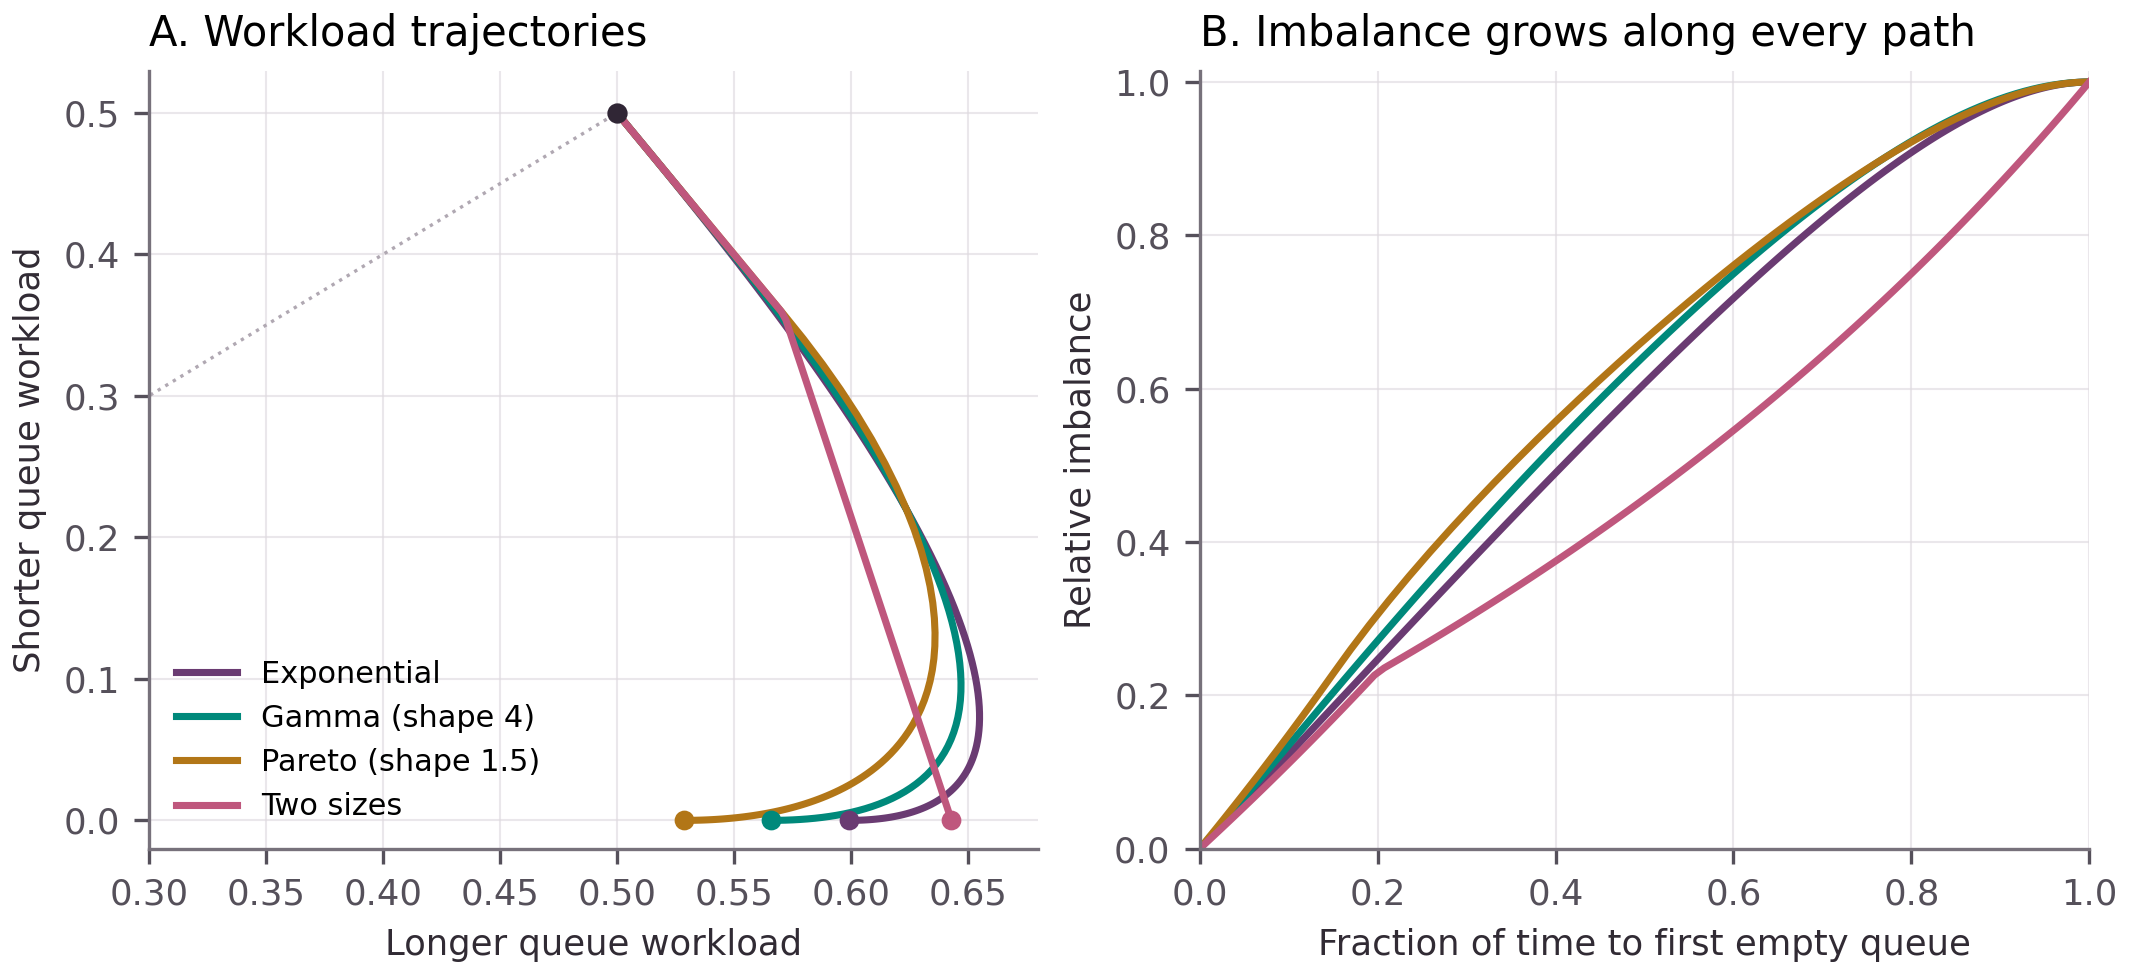
\includegraphics[width=\linewidth]{optimal_paths.png}
\caption{Optimal paths at $\rho=3/4$ from $(1/2,1/2)$ for four laws. Left: workloads. Right: relative imbalance against time, with time normalised by each path's first-axis time. Theorem~\ref{thm:monotone} proves the increase for every optimal path; the curves only illustrate it.}\label{fig:paths}
\end{figure}

\begin{thebibliography}{99}\small\raggedright
\bibitem{ABR1995} F.~Avram, D.~Bertsimas and M.~Ricard. Fluid models of sequencing problems in open queueing networks; an optimal control approach. In \emph{Stochastic Networks}, IMA Vol.\ Math.\ Appl.\ 71, Springer, 1995, 199--234. doi:10.1007/978-1-4757-2418-9\_11.
\bibitem{AKLL2018} I.~J.~B.~F.~Adan, V.~G.~Kulkarni, N.~Lee and E.~Lefeber. Optimal routeing in two-queue polling systems. \emph{J.\ Appl.\ Probab.} 55(3) (2018) 944--967. doi:10.1017/jpr.2018.59.
\bibitem{BCD1997} M.~Bardi and I.~Capuzzo-Dolcetta. \emph{Optimal Control and Viscosity Solutions of Hamilton--Jacobi--Bellman Equations}. Birkh\"auser, 1997. doi:10.1007/978-0-8176-4755-1.
\bibitem{Bauerle2000} N.~B\"auerle. Asymptotic optimality of tracking policies in stochastic networks. \emph{Ann.\ Appl.\ Probab.} 10(4) (2000) 1065--1083. doi:10.1214/aoap/1019487606.
\bibitem{BMDP2002} A.~Bemporad, M.~Morari, V.~Dua and E.~N.~Pistikopoulos. The explicit linear quadratic regulator for constrained systems. \emph{Automatica} 38(1) (2002) 3--20. doi:10.1016/S0005-1098(01)00174-1.
\bibitem{FMR2005} H.~Feng, V.~Misra and D.~Rubenstein. Optimal state-free, size-aware dispatching for heterogeneous M/G/-type systems. \emph{Perform.\ Eval.} 62(1--4) (2005) 475--492. doi:10.1016/j.peva.2005.07.031.
\bibitem{FS2006} W.~H.~Fleming and H.~M.~Soner. \emph{Controlled Markov Processes and Viscosity Solutions}, 2nd ed. Springer, 2006. doi:10.1007/0-387-31071-1.
\bibitem{HB2013} M.~Harchol-Balter. \emph{Performance Modeling and Design of Computer Systems}. Cambridge University Press, 2013. doi:10.1017/CBO9781139226424.
\bibitem{HCM1999} M.~Harchol-Balter, M.~E.~Crovella and C.~D.~Murta. On choosing a task assignment policy for a distributed server system. \emph{J.\ Parallel Distrib.\ Comput.} 59(2) (1999) 204--228. doi:10.1006/jpdc.1999.1577.
\bibitem{HPA2012} E.~Hyyti\"a, A.~Penttinen and S.~Aalto. Size- and state-aware dispatching problem with queue-specific job sizes. \emph{European J.\ Oper.\ Res.} 217(2) (2012) 357--370. doi:10.1016/j.ejor.2011.09.029.
\bibitem{HR2022} E.~Hyyti\"a and R.~Righter. On sequential dispatching policies. In \emph{32nd Int.\ Telecommunication Networks and Applications Conf.\ (ITNAC)}, 2022, 1--6. doi:10.1109/ITNAC55475.2022.9998339.
\bibitem{HR2024} E.~Hyyti\"a and R.~Righter. Towards the optimal dynamic size-aware dispatching. \emph{Perform.\ Eval.} 164 (2024) 102396. doi:10.1016/j.peva.2024.102396.
\bibitem{Maglaras2000} C.~Maglaras. Discrete-review policies for scheduling stochastic networks: trajectory tracking and fluid-scale asymptotic optimality. \emph{Ann.\ Appl.\ Probab.} 10(3) (2000) 897--929. doi:10.1214/aoap/1019487513.
\bibitem{Meyn2008} S.~Meyn. \emph{Control Techniques for Complex Networks}. Cambridge University Press, 2008. doi:10.1017/CBO9780511804410.
\bibitem{MV2022} M.~Mitzenmacher and S.~Vassilvitskii. Algorithms with predictions. \emph{Commun.\ ACM} 65(7) (2022) 33--35. doi:10.1145/3528087.
\bibitem{SGM2022} Z.~Scully, I.~Grosof and M.~Mitzenmacher. Uniform bounds for scheduling with job size estimates. In \emph{13th Innovations in Theoretical Computer Science Conf.\ (ITCS 2022)}, LIPIcs 215, 114:1--114:30. doi:10.4230/LIPIcs.ITCS.2022.114.
\bibitem{SS2007} M.~Shaked and J.~G.~Shanthikumar. \emph{Stochastic Orders}. Springer, 2007. doi:10.1007/978-0-387-34675-5.
\bibitem{Soner1986} H.~M.~Soner. Optimal control with state-space constraint I. \emph{SIAM J.\ Control Optim.} 24(3) (1986) 552--561. doi:10.1137/0324032.
\bibitem{vEHvL2022} W.~van Eekelen, D.~den Hertog and J.~S.~H.~van Leeuwaarden. MAD dispersion measure makes extremal queue analysis simple. \emph{INFORMS J.\ Comput.} 34(3) (2022) 1681--1692. doi:10.1287/ijoc.2021.1130.
\bibitem{Villani2009} C.~Villani. \emph{Optimal Transport: Old and New}. Springer, 2009. doi:10.1007/978-3-540-71050-9.
\bibitem{Weiss2008} G.~Weiss. A simplex based algorithm to solve separated continuous linear programs. \emph{Math.\ Program.} 115 (2008) 151--198. doi:10.1007/s10107-008-0217-x.
\bibitem{Winston1977} W.~Winston. Optimality of the shortest line discipline. \emph{J.\ Appl.\ Probab.} 14(1) (1977) 181--189. doi:10.2307/3213271.
\bibitem{XGS2024} R.~Xie, I.~Grosof and Z.~Scully. Heavy-traffic optimal size- and state-aware dispatching. \emph{Proc.\ ACM Meas.\ Anal.\ Comput.\ Syst.} 8(1) (2024) Art.~9, 1--36. doi:10.1145/3639035.
\bibitem{XHR2026} R.~Xie, E.~Hyyti\"a and R.~Righter. Size-aware dispatching to fluid queues. \emph{ACM SIGMETRICS Perform.\ Eval.\ Rev.} 53(4) (2026) 42--48. doi:10.1145/3797823.3797843. Preprint arXiv:2509.21693v1.
\end{thebibliography}
\end{document}
